%======================= PREAMBOLO DICHIARAZIONI INIZIALI===============%
\documentclass[10pt,oneside,a4paper]{article}

\usepackage[latin1]{inputenc} 
\usepackage[italian]{babel}
\usepackage{siunitx} %Inserisce automaticamente i dati con le unità  di misura correttamente formattate del SI (utilizzo: \SI{0.82}{m^2}, in generale \SI{misura con il punto decimale}{unità  di misura})
\sisetup{output-decimal-marker = {.}, separate-uncertainty = true, input-uncertainty-signs = \pm, detect-weight=true, detect-family=true} %per usare SI con il punto decimale
\usepackage{listings} %Per citare codice informatico formattandolo correttamente
\usepackage{amsmath}
\usepackage{graphicx}
\usepackage{geometry}
\usepackage{epigraph}
\usepackage{booktabs}	%tabelle migliorate
\usepackage{tablefootnote}	%note a piè di pagina in tabella
\usepackage{threeparttable} %tabella con note a piè di tabella
\usepackage{caption}	%descrizione per figure
\captionsetup{tableposition=top,figureposition=bottom,font=small} %setup descrizione
\usepackage{float}
\usepackage{esvect} %vettori
\usepackage{longtable} %tabelle lunghe
\usepackage[dvipsnames]{xcolor}
\definecolor{sepia}{HTML}{80002A}
\usepackage[colorlinks=true, citecolor=black, linkcolor=sepia, urlcolor=black]{hyperref}
\usepackage{mathrsfs}

\usepackage{listings} %Per inserire codice
\lstnewenvironment{codice_c}[1][]
{\lstset{basicstyle=\small\ttfamily, columns=fullflexible,
keywordstyle=\color{red}\bfseries, commentstyle=\color{blue},
language=C, basicstyle=\small,
numbers=left, numberstyle=\tiny,
stepnumber=2, numbersep=5pt, frame=shadowbox, #1}}{}

\setcounter{section}{-1}

%========= PRIMA PAGINA ===========%
\title{\textsc{Misura della frequenza di fenomeni radioattivi e studio di un pallinometro}}
\author{\small{G. Galbato Muscio} \and \small{L. Gravina} \and \small{L. Graziotto} \and \small{M. Rescigno}}
\date{}

\begin{document}
	\begin{figure}
		\centering
		
\includegraphics[scale=0.5, trim={2.8cm 8.9cm 0 9cm}, clip]{logo.png}
	\end{figure}
	\maketitle
	\begin{center} 
		\fbox{{\fontsize{12pt}{8mm}\textsc{Gruppo B2.3}}} \\
		\vspace{1cm}
		\begin{tabular}{ccc}
			Esperienza di laboratorio && Consegna della relazione \\
			\emph{\small{3 maggio 2017}} && \emph{\small{14 maggio 2017}} \\
		\end{tabular} 
		
		\vspace{0.5cm}
		
	\end{center}
\hrule
\vspace{0.5cm}
\begin{abstract}
Utilizzando un contatore Geiger-M\"uller misuriamo la radioattività  ambientale, quella dovuta ai raggi cosmici e la radiazione emessa da un blocco di tufo. Studiamo quindi la distribuzione delle biglie in un pallinometro fisico e in uno simulato.	
\end{abstract}
\newpage
\tableofcontents %Indice
\listoftables %Indice delle tabelle
\listoffigures %Indice dei grafici
\pagebreak
\section{Convenzioni e formule}
In questa relazione verranno usate le seguenti convenzioni:
\begin{enumerate}
	\item sarà usato il punto [ $.$ ] come separatore decimale;
	\item l'approssimazione decimale della cifra $5$ sarà fatta per eccesso;
	\item al fine di snellire la relazione e migliorarne la leggibilità , riporteremo nel corpo del documento solamente le tabelle riepilogative e alcuni grafici, e dedicheremo un'appendice finale alle tabelle e ai grafici più dettagliati.
\end{enumerate}
Inoltre, si farà riferimento alle seguenti formule:
\begin{enumerate}
	\item media 
	\begin{equation}\label{eq:media}
	\bar{x} = \frac{1}{N}\sum_{i=1}^Nx_i;
	\end{equation}
	\item varianza
	\begin{equation}\label{eq:varianza}
	\sigma^2 = \frac{1}{N}\sum_{i=1}^N(x_i-\bar{x})^2;
	\end{equation}
	\item deviazione standard
	\begin{equation}\label{eq:deviazione}
	\sigma = \sqrt{\sigma^2}.
	\end{equation}	
\end{enumerate}

%===============SCOPO E DESCRIZIONE DELL'ESPERIENZA==============%
\section{Scopo e descrizione dell'esperienza}
\label{sec:descrizione}
\paragraph{Misura di fenomeni di radiazione}
L'evento ``osservazione di una particella radioattiva'' è descritto da una distribuzione di probabilità  poissoniana; fissato un intervallo di tempo $\Delta t$, il parametro della distribuzione è $\lambda = R\Delta t$, ove $R$ indica il valore atteso del numero di conteggi per unità  di tempo. La distribuzione di probabilità  della variabile $x$, indicante il numero di conteggi, è data dall'equazione
\begin{equation}\label{eq:Poisson}
f(x\vert \mathcal{P}_{\lambda}) = \frac{\lambda^x}{x!}e^{-\lambda},
\end{equation}
ed ha valore atteso $\lambda$ e deviazione standard $\sqrt{\lambda}$.
Interessandoci invece al tempo di attesa per rilevare una particella radioattiva, la probabilità  che il primo conteggio avvenga dopo l'intervallo di tempo $\Delta t$ è data da
\[
P(T > \Delta t) = e^{-\Delta t / \tau},
\]
ove il rapporto $\Delta t / \tau$ è pari al parametro $\lambda$ della precedente distribuzione di Poisson, e si è introdotto il parametro $\tau = 1 / R$ quale previsione del tempo di attesa prima che si verifichi il primo conteggio. 

A partire dalle misure sperimentali è possibile inferire il parametro $\lambda$ della distribuzione che descrive (nel nostro modello) il decadimento radioattivo: per intervalli di tempo brevi ($\Delta t < \SI{5}{s}$) il numero di conteggi sarebbe troppo basso per rendere legittima l'approssimazione gaussiana della poissoniana, però, avendo fatto $N = 50$ misure tra loro equivalenti, è legittimo considerare le $N$ misure dell'intervallo $\Delta t$ come un'unica misura di un intervallo $N \Delta t$, il numero di conteggi diventa quindi $\sum_{i=1}^N x_i$ (con $x_i$ il numero di conteggi nella misura $i$-esima) e di conseguenza l'approssimazione gaussiana diventa legittima. Invertendo la gaussiana che ora descrive il nostro modello si ottiene la distribuzione del parametro $\lambda$:
\begin{equation}\label{eq:distribuzione_lambda}
	\lambda[\Delta t]  \sim \mathscr{N} \left( \frac{\sum_{i=1}^N x_i}{N} , \frac{\sqrt{\sum_{i=1}^N x_i}}{N} \right) = \mathscr{N} \left( \bar{x}, \sqrt{\frac{\bar{x}}{N}} \right)
\end{equation}
dove $x_i$ è, come prima, il numero di conteggi nella $i$-esima misura. Da questa distribuzione segue quella del \emph{rate} della distribuzione:
\begin{equation}\label{eq:distribuzione_r}
	r \sim \mathscr{N} \left( \frac{\bar{x}}{\Delta t}, \sqrt{\frac{\bar{x}}{(\Delta t)^2 N}} \right),
\end{equation}
per cui la migliore stima di $r$ è
\begin{equation}\label{eq:stima_r}
	r = \mathrm{E}[r] \pm \sigma [r]
\end{equation} dove
\[
	\mathrm{E}[r] = \frac{\bar{x}}{\Delta t}, \qquad \sigma [r] = \sqrt{\frac{\bar{x}}{(\Delta t)^2 N}}.
\]
\paragraph{Studio di un pallinometro}
Il pallinometro è uno strumento utilizzato per verificare le proprietà  della distribuzione binomiale, in cui alcune sferette vengono inserite in cima ad esso e, dopo aver colpito $N-1$ file di chiodi con probabilità  $p$ di andare dopo l'urto a destra e con probabilità  $1-p$ di andare invece a sinistra, cadono all'interno di $N$ cellette. Studiamo l'andamento della distribuzione delle palline sia utilizzando un pallinometro fisico sia una simulazione via software.


%================APPARATO SPERIMENTALE======================%		
\section{Apparato Sperimentale}
	
\subsection{Strumenti}
\label{subsec:strumenti}
\begin{itemize}
\item Contatore Geiger-M\"uller (Integrated Pancake Frisker - Model 26) [superficie sensibile: \SI{15}{cm^2}];
\item Livella digitale [digit: \SI{1}{°}];
\item Software \emph{Palli2000} che simula il pallinometro.
\end{itemize}

\subsection{Materiali}
\begin{itemize}
\item Blocco di tufo;
\item Pallinometro fisico [33 file di chiodi, 34 bin].
\end{itemize}


%==================SEQUENZA OPERAZIONI SPERIMENTALI==========
\section{Sequenza Operazioni Sperimentali} 

\subsection{Misura dei conteggi per unità  di tempo con un contatore Geiger-M\"uller}
\subsubsection{Misura dei conteggi per unità  di tempo del fondo}
Utilizziamo il contatore Geiger-M\"uller in modalità  \textbf{scaler}, in cui si acquisisce il numero di conteggi di particelle radioattive che attraversano il rilevatore per un fissato intervallo di tempo $\Delta t$. Posizioniamo il contatore sul tavolo in orizzontale, ad una distanza superiore ai \SI{70}{cm} dal blocco di tufo. Ripetiamo per $50$ volte la misura del numero di conteggi per intervalli di tempo $\Delta t$ pari a: $\Delta t_1 = \SI{1}{s}$, $\Delta t_2 = \SI{2}{s}$, $\Delta t_3 = \SI{3}{s}$, $\Delta t_4 = \SI{4}{s}$, $\Delta t_5 = \SI{10}{s}$.

Il numero di conteggi per i diversi intervalli di tempo è riportato in tabella~\ref{tab:conteggi_tempo} e negli istogrammi di figura~\ref{fig:istogramma_deltat1}, \ref{fig:istogramma_deltat2}, \ref{fig:istogramma_deltat3}, \ref{fig:istogramma_deltat4} e \ref{fig:istogramma_deltat5}.
\paragraph{Stima di lambda per i diversi intervalli temporali}
Per quanto detto nella sezione~\ref{sec:descrizione}, stimiamo i parametri $\lambda_i$ della distribuzione di Poisson relativa ai diversi intervalli temporali calcolando il valor medio del numero di conteggi acquisiti per i diversi $\Delta t_i$. A tali stime associamo come incertezza il secondo parametro della distribuzione (\ref{eq:distribuzione_lambda}). Da queste stime, utilizzando la distribuzione descritta in (\ref{eq:distribuzione_r}), seguono le stime dei relativi tassi di conteggio con relative incertezze: riportiamo le stime di $\lambda_i$  e di $r$ in tabella~\ref{tab:lambda_r_conteggi}.
\begin{table}[ht]
\caption{Stime di $\lambda$ e di $r$ per diversi intervalli temporali}
\label{tab:lambda_r_conteggi}
\centering
\begin{tabular}{c|cc|cc}
\toprule
Intervallo [\SI{}{s}] & $\lambda$ & $\sigma_{\lambda}$ & $r$ & $\sigma_{r}$ \\
\hline 
$\Delta t_1 = 1$ & 0.80  & 0.13 & 0.80 & 0.13\\ 
$\Delta t_2 = 2$ & 1.9  & 0.2 & 0.97 & 0.10\\
$\Delta t_3 = 3$ & 3.3  & 0.3  & 1.11 & 0.09\\
$\Delta t_4 = 4$ & 3.7  & 0.3 & 0.93 & 0.07\\
$\Delta t_5 = 10$ & 10.6 & 0.5 & 1.06 & 0.04\\
\bottomrule
\end{tabular}
\end{table}
\paragraph{Stima di $r_\mathrm{best}$}
I tassi di conteggio al secondo risultano compatibili a meno di inevitabili fluttuazioni statistiche, ma possiamo migliorare la stima di $r$ combinando tutte le misure prese: è legittimo considerare le $5 N = 250$ misure di conteggio relative a diversi intervalli temporali come un'unica misura di un intervallo di tempo $\Delta t = N ( \Delta t_1 + \Delta t_2 + \Delta t_3 + \Delta t_4 + \Delta t_5)$ con numero di conteggi associato pari a alla somma di tutti i conteggi, in questo modo il parametro $r_\mathrm{best}$ si stima come
\begin{equation}\label{eq:stima_r_tot}
	r_\mathrm{best} = \mathrm{E}[r_\mathrm{best}] \pm \sigma [r_\mathrm{best}]
\end{equation} dove
\[
	\mathrm{E}[r_\mathrm{best}] = \frac{x_{\mathrm{tot}} +1}{\Delta t} \approx \frac{x_{\mathrm{tot}}}{\Delta t}, \quad \sigma[r_\mathrm{best}] = \frac{\sqrt{x_{\mathrm{tot}} +1}}{\Delta t} \approx  \sqrt{\frac{\mathrm{E}[r_\mathrm{best}]}{\Delta t}},
\] svolgendo i conti segue che la miglior stima del tasso di conteggio nelle condizioni in cui si è svolta l'esperienza è 
\[
	\boxed{\textbf{$r_\mathrm{best}$ = {\SI{1.02 \pm 0.03}{\frac{conteggi}{s}}}}}.
\]

\paragraph{Test del $\mathbf{Chi}^2$}Sovrapponendo a ciascun istogramma l'andamento atteso per una distribuzione di Poisson con parametro $\lambda_i = r_{\mathrm{best}} \Delta t_i$ notiamo che entro le barre di incertezza i dati sono compatibili quasi ovunque. Inoltre osserviamo che all'aumentare del tempo di osservazione l'andamento della distribuzione delle frequenze dei conteggi tende alla distribuzione gaussiana, dalla caratteristica simmetria già  parzialmente visibile per $\Delta t_5 = \SI{10}{s}$. Le barre di incertezza hanno lunghezza data dalla radice del numero di conteggi, e sono state attribuite ai punti teorici invece che al numero di conteggi in quanto l'esperienza condotta si pone lo scopo di risalire alla forma della distribuzione a partire dal numero (noto) di conteggi, e infatti il parametro della distribuzione di Poisson che rappresenta l'andamento teorico è stato inferito proprio dai valori sperimentali.

Per valutare se i dati sperimentali risultano in accordo con il modello teorico, calcoliamo il $\chi^2$ relativo ad ogni istogramma attraverso l'equazione
\begin{equation}\label{eq:chi2}
	\chi^2 = \sum_{i=1}^{N_\mathrm{bin}} \frac{(n_i - N p_i)^2}{N p_i ( 1 - p_i)}
\end{equation}
dove $N = 50$ è il numero di misure prese, $n_i$ il numero di conteggi nell'$i$-esimo bin e $p_i$ la probabilità rispetto all'$i$-esimo bin data da una distribuzione di Poisson di \emph{rate} pari a $r_{\mathrm{best}}$ calcolata nel punto centrale del bin: affinché il test risulti valido è necessario che $Np_i$ sia sufficientemente grande, in modo da poter approssimare la distribuzione ad una gaussiana, a tal fine quando la probabilità del bin è minore di $0.1$ si considera un bin più largo dato dall'unione di due (o più) bin contigui, il numero di conteggi diventa quindi la somma di quelli nei rispettivi bin e la probabilità diventa la somma delle rispettive probabilità. I valori del $\chi^2$ per ciascun istogramma sono riportati in tabella \ref{tab:chi2}, nell'ultima colonna sono riportati i gradi di fiducia che la distribuzione sperimentale provenga da una distribuzione di Poisson di parametro noto (il grado di fiducia coincide con la probabilità di ottenere un $\chi^2$ maggiore ripetendo l'esperimento; la distribuzione usata è quella del $\chi^2$ con numero di gradi di libertà pari al numero di bin\footnote{Infatti la distribuzione di conteggi non ha alcun vincolo formale.}).
\begin{table}[t]
\caption{Test del $\mathrm{Chi}^2$ sui conteggi di radioattività}
\label{tab:chi2}
\centering
\begin{tabular}{ccc}
\toprule
Intervallo [\SI{}{s}] & $\chi^2$ & p\\
\hline 
$\Delta t_1 = 1$ &  3.224 & 0.86\\  %Bisogna rifare i conti per tutti gli intervalli (eccetto per l'ultimo)
$\Delta t_2 = 2$ & 1.425 & 0.98\\
$\Delta t_3 = 3$ & 3.856 & 0.85\\
$\Delta t_4 = 4$ & 6.146 & 0.80\\
$\Delta t_5 = 10$ & 8.504 & 0.99\\
\bottomrule
\end{tabular}
\end{table}

I risultati del test mostrano che i dati sperimentali sono ben compatibili con il modello di una poissoniana: il risultato migliore si è avuto, com'era prevedibile, con la misura nell'intervallo di tempo più grande. I valori piuttosto bassi ottenuti per gli altri intervalli (eccezion fatta per $\Delta t_2$) sono giustificati se si ricorda che il test del $\chi^2$ è significativo per misure in cui sono stati rilevati un numero considerevole di eventi (almeno maggiore di 30), per cui l'unico test effettivamente significativo è quello con $\Delta t = \SI{10}{s}$. 

\paragraph{Rappresentazione della funzione di verosimiglianza}
Per calcolare la funzione di verosimiglianza del tasso di conteggio per i tre diversi intervalli temporali $\Delta t_1= \SI{1}{s}$, $\Delta t_2= \SI{4}{s}$, $\Delta t_3= \SI{600}{s}$, combiniamo le $n$ misure di conteggio moltiplicando la densità  di probabilità del tasso di conteggio $r$ di ogni singola misura, ottenuta applicando il procedimento bayesiano. La funzione cercata sarà quindi, a meno di fattori moltiplicativi di normalizzazione:
\begin{equation}\label{eq:verosimiglianzatempiuguali}
f(\lambda|x) \propto \lambda^{ \sum_{i}x_i}\cdot e^{n\lambda}
\end{equation}
Dove $n$ è il numero di osservazioni di ciascun gruppo e $x_i$ sono i conteggi dell'osservazione $i$-esima.
I grafici \ref{fig:verosimiglianza1sec}, \ref{fig:verosimiglianza4sec}, \ref{fig:verosimiglianza600sec} rappresentano le funzioni di verosimiglianza, non normalizzate, rispettivamente per gli intervalli temporali $\Delta t_1= \SI{1}{s}$, $\Delta t_2= \SI{4}{s}$ e $\Delta t_3= \SI{600}{s}$. Notiamo che i punti di massimo di tali funzioni sono vicini tra di loro e la sovrapposizione delle tre funzioni di verosimiglianza è significativa, indicando che le tre misure indipendenti sono tra di loro compatibili.
Per quanto riguarda la combinazione di tutte le misure, poiché stiamo studiando uno stesso fenomeno ma osservato in diversi intervalli temporali, la funzione, a meno di fattori moltiplicativi è data da: 
\begin{equation}\label{eq:verosimiglianzatempidiversi}
f(r|x) \propto r^{\sum_{i}x_i} \cdot e^{-r\sum_{i}T_i}
\end{equation}
La macro fornita come esempio non gestisce correttamente tale calcolo, dovendo calcolare esplicitamente funzioni esponenziali con argomenti molto grandi. Il grafico \ref{fig:verosimiglianzacombinata} è ottenuto quindi modificando la macro di esempio per calcolare la funzione $g(x)=-\mathrm{ln}(f(r|x))$, che è più facilmente calcolabile dal calcolatore. Il valore più probabile che nella rappresentazione grafica precedente corrisponde con il massimo nella funzione, in questo caso corrisponde al minimo. Tale valore, che corrisponde a circa $1.05$, è compatibile con la nostra stima di $r_\mathrm{best}$.


\paragraph{Frazione di 0 e 0+1 conteggi} 
Escludendo il set di dati relativo a $\Delta t_5$, calcoliamo la frazione di $0$ conteggi e di $0$ o $1$ conteggio, riportata in tabella~\ref{tab:0e01conteggi}. Introduciamo il parametro $\tau = 1/R$ indicante la previsione del tempo di attesa prima che si verifichi il primo conteggio. Per quanto riguarda la prima frazione, essa ci permette di stimare l'andamento della probabilità  che il primo conteggio si verifichi dopo un intervallo di tempo $\Delta t$, ed equivale alla differenza tra $1$ e la funzione di ripartizione del tempo di attesa per un conteggio, ossia
\[
F(\Delta t) = e^{-\frac{\Delta t}{\tau}} = e^{-R\Delta t}.
\]
Sovrapponiamo dunque al grafico, in figura~\ref{fig:0conteggi}, delle frazioni di $0$ conteggi in funzione di $\Delta t$ l'andamento aspettato previsto dalla distribuzione esponenziale dei tempi di attesa, descritto dalla equazione precedente, dove abbiamo utilizzato come \emph{rate} quella estratta nella successiva sezione~\ref{subsec:10minuti} a partire dai conteggi con contatore orizzontale per il fondo. Come incertezza notiamo che l'errore qui associato è di tipo binomiale, poiché consideriamo come \emph{successo} il numero di conteggi pari a $0$ e \emph{insuccesso} l'evento complementare. Pertanto, si ha
\begin{equation}\label{eq:errorbarsgeiger}
\sigma_{\text{$0$ conteggi}} = \sqrt{\frac{p\cdot(1-p)}{N}},
\end{equation}
ove come probabilità  $p$ scegliamo la frequenza relativa dei casi con $0$ conteggi, ed $N$ è pari a $50$. Riportiamo tale incertezza come barre di errore nel grafico prima citato.

Per quanto riguarda invece la seconda frazione, essa corrisponde alla distribuzione del tempo di attesa per il secondo conteggio, ossia alla probabilità  di osservare $0$ o $1$ conteggio nell'intervallo di tempo $\Delta t$. La funzione che descrive questa probabilità  è
\[
G(\Delta t) = e^{-\frac{\Delta t}{\tau}} + \frac{\Delta t}{\tau} e^{-\frac{\Delta t}{\tau}}.
\]
Riportiamo anche in questo caso i valori ottenuti nel grafico di figura~\ref{fig:0+1conteggi}, sovrapponendo l'andamento atteso descritto dalla funzione $G(\Delta t)$, utilizzando come \emph{rate} la medesima utilizzata precedentemente, e ricordando la relazione $\tau = 1 / R$. Le incertezze sono state calcolate con la stessa equazione~\ref{eq:errorbarsgeiger}, utilizzando ancora come probabilità  $p$ la frequenza relativa dei casi con $0$ e con $1$ conteggio, derivante dal fatto che l'errore sia ancora di tipo binomiale, considerando come \emph{successo} il numero di conteggi pari a $0$ o $1$. Anche in questo caso l'incertezza è rappresentata con le barre di errore.

Notiamo che entro le barre di incertezza le nostre misure sono compatibili con la distribuzione teorica prevista per i tempi di attesa. Calcoliamo dunque il chi quadro per quantificare tale compatibilità, utilizzando nel primo caso l'equazione
\[
\chi^2 = \sum_{i = 1}^4 \frac{\big(f_0(\Delta t_i) - Np_i\big)^2}{Np_i(1-p_i)} = \sum_{i = 1}^4 \frac{\big(f_0(\Delta t_i) - N\cdot e^{-r_{\text{best}}\Delta t_i}\big)^2}{Ne^{-r_{\text{best}}\Delta t_i}(1-e^{-r_{\text{best}}\Delta t_i})}
\]
dove con $f_0(\Delta t_i)$ abbiamo indicato la frazione di $0$ conteggi relativa all'intervallo di tempo $\Delta t_i$. Otteniamo il valore $\chi^2 = 1.77$ per i dati relativi alla frazione di $0$ conteggi.

Allo stesso modo, nel caso di $0+1$ conteggi utilizziamo l'equazione
\[
\chi^2 = \sum_{i = 1}^4 \frac{\big(f_{0+1}(\Delta t_i) - Np_i\big)^2}{Np_i(1-p_i)} = \sum_{i = 1}^4 \frac{\left(f_{0+1}(\Delta t_i) - N\cdot e^{-r_{\text{best}}\Delta t_i}(1+r_{\text{best}}\Delta t)\right)^2}{Ne^{-r_{\text{best}}\Delta t_i}(1+r_{\text{best}}\Delta t)\big(1-e^{-r_{\text{best}}\Delta t_i}(1+r_{\text{best}}\Delta t)\big)}
\]
e ricaviamo $\chi^2 = 4.51$.

\begin{table}[ht]
\caption{Frazione di $0$ e di $0+1$ conteggi negli intervalli tra $1$ e \SI{4}{s}}
\label{tab:0e01conteggi}
\centering
\begin{tabular}{ccc}
\toprule
Intervallo & Frazione di 0 conteggi & Frazione di 0 e di 1 conteggi \\
\hline 
$\Delta t_1$ & 0.42  & 0.84 \\ 
$\Delta t_2$ & 0.12  & 0.42 \\
$\Delta t_3$ & 0.02  & 0.14 \\
$\Delta t_4$ & 0.02  & 0.06 \\
\bottomrule
\end{tabular}
\end{table}

\subsubsection{Misura dei conteggi per unità  di tempo del fondo e del blocco di tufo}
\label{subsec:10minuti}
Utilizzando ancora il contatore Geiger-M\"uller in modalità  \textbf{scaler}, acquisiamo i conteggi per un intervallo di tempo di $\Delta t = \SI{600}{s}$, ponendolo prima orizzontale e lontano dal blocco di tufo, quindi verticale, ossia inclinato su un fianco, infine appoggiato sul blocco di tufo. I conteggi misurati sono riportati in tabella~\ref{tab:conteggi600s}.

\begin{table}[ht]
\caption{Conteggi acquisiti in un intervallo temporale di \SI{600}{s}}
\label{tab:conteggi600s}
\centering
\begin{tabular}{ccc}
\toprule
Contatore orizzontale & Contatore verticale & Contatore sul blocco di tufo \\
\hline 
646 & 588 & 1395 \\
\bottomrule
\end{tabular}
\end{table}

Dai conteggi misurati è possibile stimare i parametri di Poisson $\lambda$, con incertezza data da $\sqrt{\lambda}$. Si ha dunque
\begin{align*}
\hat{\lambda}_{\text{ambiente+raggi cosmici}} &= \hat{\lambda}_{A+C} = 646 \pm \sqrt{646} \\
\hat{\lambda}_{\text{ambiente+$\frac{1}{2}$raggi cosmici}} &= \hat{\lambda}_{A+\frac{1}{2}C} = 588 \pm \sqrt{588} \\
\hat{\lambda}_{\text{ambiente+raggi cosmici+ tufo}} &= \hat{\lambda}_{A+C+T} = 1395 \pm \sqrt{1395}, 
\end{align*}
ricordando che ponendo il Geiger in posizione verticale misuriamo all'incirca la metà  dei raggi cosmici misurati nella configurazione orizzontale. Possiamo ora calcolare i parametri di Poisson che otterremmo se potessimo misurare solo la radioattività  ambientale: 
\[
\hat{\lambda}_A = 2\cdot\hat{\lambda}_{A+\frac{1}{2}C}-\hat{\lambda}_{A+C} = 530 \pm 55,
\]
dove l'incertezza è stata propagata con la formula
\[
\sigma_{\hat{\lambda}_A} = \sqrt{\left(2\cdot\sigma_{\hat{\lambda}_{A+\frac{1}{2}C}}\right)^2+\sigma_{\hat{\lambda}_{A+C}}^2};
\]
i raggi cosmici:
\[
\hat{\lambda}_C = 2\cdot (\hat{\lambda}_{A+C} - \hat{\lambda}_{A+\frac{1}{2}C}) = 116 \pm 70,
\]
dove l'incertezza è stata propagata con la formula
\[
\sigma_{\hat{\lambda}_C} = 2\cdot\sqrt{\sigma_{\hat{\lambda}_{A+C}}^2+\sigma_{\hat{\lambda}_{A+\frac{1}{2}C}}^2};
\]
e la radioattività  del tufo:
\[
\hat{\lambda}_T = \hat{\lambda}_{A+C+T} - \hat{\lambda}_{A+C} = 749 \pm 45,
\]
dove l'incertezza è stata propagata con la formula
\[
\sigma_{\hat{\lambda}_{T}} = \sqrt{\sigma_{\hat{\lambda}_{A+C+T}}^2+\sigma_{\hat{\lambda}_{A+C}}^2}.
\]
Come detto nella sezione~\ref{sec:descrizione}, il parametro di Poisson è legato al \emph{rate} $r$, ossia al numero di conteggi per unità  di tempo, dall'equazione $\lambda = r\Delta t$, dove $\Delta t$ è pari nel nostro caso a \SI{600}{s}, con incertezza trascurabile rispetto a quella sul numero di conteggi. Dai valori precedenti di lambda otteniamo dunque per la radioattività  ambientale un \emph{rate} pari a
\[
r_A = \frac{\hat{\lambda}_A}{\Delta t} = \SI{0.88 \pm 0.09}{s^{-1}},
\] 
per i raggi cosmici un valore di
\[
r_C = \frac{\hat{\lambda}_C}{\Delta t} = \SI{0.19 \pm 0.12}{s^{-1}},
\]
e per la radioattività  del tufo
\[
r_T = \frac{\hat{\lambda}_T}{\Delta t} = \SI{1.25 \pm 0.07}{s^{-1}}.
\]
Le incertezze, data la trascurabilità  di quella sul tempo, sono state ottenute dividendo quelle del parametro di Poisson per l'intervallo di tempo.
Notiamo che le incertezze relative sono maggiori del $5\%$ e, nel caso dei raggi cosmici, arrivano a superare il $63\%$: riteniamo che questo sia dovuto al fatto che abbiamo eseguito una sola misurazione della radiazione e compiuto l'analisi di un solo dato; riteniamo che avendo preso la media di più misurazioni l'incertezza sarebbe diminuita. Inoltre sottolineiamo che non abbiamo considerato il possibile rumore elettronico del contatore Geiger-M\"uller, che potrebbe aver influito sul conteggio di alcuni eventi non realmente rilevati.

Per confronto con la prima parte di questa sezione dedicata al conteggio di fenomeni di radiazione, notiamo che dalle misure riportate nella tabella~\ref{tab:lambda_r_conteggi} possiamo estrarre un \emph{rate} medio per la radiazione di fondo, comprendente quella ambientale e i raggi cosmici, pari a $R = \SI{0.98 \pm 0.12}{s^{-1}}$, con incertezza data dalla deviazione standard dei valori del rate ricavati dalla tabella indicata ($R = \lambda / \Delta t$). Questo valore è compatibile entro un sigma con quello ricavato poco sopra, dunque possiamo concludere che i risultati ottenuti misurando la radiazione per intervalli inferiori o uguali a \SI{10}{s} siano in accordo con quelli ottenuti con l'intervallo temporale di \SI{600}{s}, in quanto la distribuzione di probabilità  sottostante al fenomeno è la stessa.


\subsection{Pallinometro}\label{sec:pallinometro}
\begin{figure}[h]
\centering
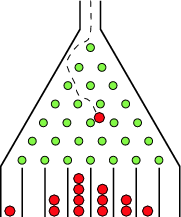
\includegraphics{pallinometro.png}
\caption{Schematizzazione della quinconce di Galton}
\label{fig:pallinometro}
\end{figure}
Supponiamo di lasciar cadere una sferetta ideale di massa non nulla in uno strumento (anch'esso ideale) come quello in figura \ref{fig:pallinometro}: per ogni riga la sfera urterà  perfettamente verticale un chiodo (punti verdi della figura) e cadrà  con uguale probabilità  a destra o a sinistra terminando la caduta in una delle colonne sul fondo dello strumento; supponiamo quindi di ripetere l'esperienza $N$ volte: è di interesse discutere la modalità  con cui le $N$ sfere si distribuiranno nelle colonne. Lo strumento appena descritto è chiamato (a seguito del suo ideatore) \emph ``quinconce di Galton"\footnote{Per ``quinconcè' si intende il simbolo usato dai Romani per indicare la frazione $5/12$, simbolo che ricorda la disposizione dei chiodi dello strumento; volgarmente quest'ultimo è ricordato come ``pallinometro''.} ed ha le seguenti caratteristiche:
\begin{itemize}
	\item ogni collisione (da ora in poi chiamata \emph{evento}) ha esclusivamente due modalità  di manifestarsi, in quanto la pallina cade o a sinistra o a destra;
	\item il numero di eventi è discreto e finito, essendoci un evento per ogni riga\footnote{La distanza tra due righe è scelta appositamente affinché avvenga questo.};
	\item la probabilità  che la pallina cada a destra (o a sinistra) è esattamente identica\footnote{Ricordando che si tratta di un \emph{gedankenexperiment}.} per ogni chiodo e rimane costante nel tempo.
\end{itemize} Nel complesso, il singolo evento di urto della pallina con un chiodo è schematizzato da un \emph{processo di Bernoulli} e l'esito dell'esperimento è descritto da una distribuzione binomiale\footnote{In realtà , la successione logica con la quale sono stati presentati gli argomenti di questa sezione è stata invertita: storicamente, Galton ha ideato questa esperienza proprio per valutare l'efficacia della distribuzione binomiale, la quinconce non ha altro scopo.}: ci aspettiamo, infatti, di trovare nell'$i-$esimo bin un numero di sfere pari a 
\begin{align}\label{eq:palli_E}
	\vec{E}(i, N, C) &= P(i) \cdot N \notag \\
		&= \begin{pmatrix} C+1 \\ i \end{pmatrix} p^i (1-p)^{C+1-i}\cdot N
\end{align}
dove $N$ è il numero di palline lasciate cadere e $C$ il numero di collisioni prima di fermarsi (che corrisponde al numero di righe). 

Nel caso di una quinconce ideale, la probabilità  di cadere da una delle due parti è esattamente \SI{0.5}, il che rende assolutamente equivalente la scelta di quale delle due direzioni definire \emph{successo}; in quel caso l'equazione (\ref{eq:palli_E}) si semplifica in
\begin{equation}\label{eq:palli_E_teorico}
	\vec{E}(i, N, C) = \begin{pmatrix} C+1 \\ i \end{pmatrix} \left(\frac{1}{2}\right)^{C+1}.
\end{equation}

Supponendo realisticamente invece che la probabilità  non sia equivalente (per via di eventuali inclinazioni, per esempio) si avrà  una distribuzione non simmetrica descritta da una binomiale $\mathscr{B}_{N, p}$ dove la probabilità  è il valore atteso della distribuzione delle frequenze relative, cioé
\begin{equation}\label{eq:palli_P_vero}
	 p = \frac{1}{C} \sum_{x=0}^{C} x \frac{N_x}{N}
\end{equation} dove con $N_x$ si è inteso il numero di palline registrate nell'$x-$esimo bin (contandoli a partire dal primo teoricamente raggiungibile).

\subsubsection{Pallinometro fisico}
Inclinando leggermente in verticale il pallinometro e avendo cura di non inclinarlo lateralmente\footnote{La posizione orizzontale dell'apparato è stata controllata verificando che le altezze di due vertici lungo i due lati fossero uguali.} si sono lasciate cadere $N = 200$ sfere di metallo dal punto più alto, le quali hanno colliso con $C_1 = 33$ chiodi prima di distribuirsi nei vari bin; ripetendo l'esperienza variando la distanza dalla base da cui lasciar cadere le palline, si sono fatte collidere le sfere prima con $C_2 = 25$ e poi con $C_3 = 17$ chiodi, riportiamo in tabella \ref{tab:palli_orizzontale} il numero di sfere accumulatosi in ciascun bin al termine di ciascuna esperienza.

Utilizzando nell'equazione (\ref{eq:palli_P_vero}) ricaviamo la probabilità  di successo (come detto, cosa definire \emph{successo} è arbitrario, da ora in poi considereremo come successo l'evento \emph{cadere verso destra})\footnote{Nel caso avessimo scelto come successo l'evento \emph{cadere verso sinistra} avremmo dovuto contare i bin a partire da destra.} calcolandola per ogni esperienza, si ottengono i valori:
\begin{align*}
	C_1 = 33 &\longrightarrow \overline{p_1} = \SI{0.44 \pm 0.12}{} \\ 
	C_2 = 25 &\longrightarrow \overline{p_2} = \SI{0.42 \pm 0.15}{} \\
	C_3 = 17 &\longrightarrow \overline{p_3} = \SI{0.46 \pm 0.16}{},
\end{align*}
dove la deviazione standard è stata calcolata come valore atteso della distribuzione dei quadrati degli scarti. La distribuzione appare leggermente decentrata verso sinistra, riteniamo che questo sia a causa di un difetto di costruzione del pallinometro (come la posizione dei chiodi o dei buchi dai quali lasciar cadere le sfere), oltretutto a posteriori possiamo giustificare quest'inclinazione non prevista anche per via dell'inclinazione del pavimento stesso: come già  notato nell'esperienza del carrello, i pavimenti del laboratorio risultano inclinati di circa \SI{1}{°}, poiché il pallinometro è stato messo in posizione orizzontale rispetto al tavolo (il quale è a sua volta orizzontale rispetto al pavimento) esso potrebbe essere stato soggetto alla stessa inclinazione della pavimentazione. Ricordiamo, inoltre, che lo strumento\footnote{Sono stati utilizzati dei libri impilati, controllando però che il lato del pallinometro che poggiava con il sostegno fosse esattamente parallelo allo spigolo al quale era appoggiato; a questo scopo è stato usato un foglio di carta millimetrata in cima alla pila per migliorare la precisione della verifica.} per mantenere in posizione fissa lo strumento non poteva garantire una precisione molto alta.

Per confrontare i dati con le distribuzioni binomiali che nel nostro modello dovrebbero descrivere gli eventi, \emph{normalizziamo} i risultati in tabella \ref{tab:palli_orizzontale} dividendo ogni conteggio per il numero di sfere complessive, in modo da ottenere per ogni bin una percentuale relativa che è, per definizione, equivalente a quella usata in (\ref{eq:palli_E}). Riportiamo nei grafici \ref{fig:palli_orizzontale_33}, \ref{fig:palli_orizzontale_25} e \ref{fig:palli_orizzontale_17} le distribuzioni delle percentuali relative confrontate con le equivalenti distribuzioni binomiali del tipo $\mathscr{B}_{i_j, p=0.5}$ dove con $i_j$ si è indicato l'indice dell'ultimo bin raggiungibile ($i_j = (C_j+1)$).

Inclinando leggermente verso destra la quinconce e ripetendo le misure si ottengono i risultati riportati nella tabella \ref{tab:palli_inclinato}, normalizzandoli e confrontandoli con quelli teorici previste dalle binomiali del tipo $\mathscr{B}_{i_k, p_k}$ si ottengono i grafici \ref{fig:palli_inclinato_33}, \ref{fig:palli_inclinato_25} e \ref{fig:palli_inclinato_17}, dove le probabilità  $p_k$ sono ottenute con lo stesso procedimento illustrato sopra, e valgono:
\begin{align*}
	& \overline{p_1} = \SI{0.55 \pm 0.14}{} \\ 
	& \overline{p_2} = \SI{0.52 \pm 0.13}{} \\
	& \overline{p_3} = \SI{0.54 \pm 0.16}{}.
\end{align*}
Come ragionevolmente previsto, la distribuzione è leggermente spostata verso destra. Lo spostamento va relazionato a quello ottenuto con la quinconce in orizzontale, infatti l'inclinazione subita dal pallinometro è stata tale da spostare la percentuale di circa $10$ punti, e non solo di $3$ come una prima interpretazione potrebbe lasciar fraintendere.

Notiamo inoltre che il dato corrispondente al bin$-31$ nella seconda misura con lo strumento inclinato, misura riportata nella seconda colonna della tabella \ref{tab:palli_inclinato}, risulta essere incompatibile con l'esperimento: il caso limite in cui la pallina fosse sempre caduta verso destra (quindi $C_2 = 25$ successi) avrebbe portato la pallina a cadere nel bin$-29$ che quindi risultava essere l'ultimo bin teoricamente raggiungibile. Riteniamo che la causa dell'incongruenza sia dovuta ad un'eccessiva inclinazione dello strumento, la quale ha portato alcune palline a compiere più di un passo verso destra senza collidere con alcun chiodo, falsando quindi la misura. Poiché, però, le probabilità  calcolate risultano consistenti e l'evento spurio è isolato, riteniamo che il fenomeno sia stato un evento piuttosto raro e che, quindi, non abbia influito significativamente  sulla distribuzione. 

\subsubsection{Pallinometro simulato}
Attraverso il software \emph{Palli2000} in dotazione, simuliamo la caduta di $N = 10^6$ palline nelle condizioni teoriche descritte all'inizio della sezione \ref{sec:pallinometro} utilizzando come probabilità  di \emph{successo} quella teorica di $0.5$, si confrontano quindi i risultati con quelli sperimentali. Si riportano nei grafici \ref{fig:palli2000_orizzontale_33}, \ref{fig:palli2000_orizzontale_25}, \ref{fig:palli2000_orizzontale_17} le frequenze simulate con \emph{Palli2000} confrontate con quelle dei dati sperimentali: com'era prevedibile, i dati simulati seguono una distribuzione gaussiana (in quanto la binomiale tende ad una gaussiana per $N \rightarrow + \infty$), ma sono ugualmente coerenti con i dati ottenuti sperimentalmente.

Si simula ora con \emph{Palli2000} il pallinometro inclinato a partire dai valori di probabilità  per i diversi fori di ingresso della pallina $0.55, 0.52, 0.54$; nei grafici \ref{fig:palli2000_inclinato_33}, \ref{fig:palli2000_inclinato_25} e \ref{fig:palli2000_inclinato_17} si confrontano le simulazioni con i dati sperimentali: i risultati sono analoghi a quelli ottenuti con il pallinometro in posizione orizzontale.

\section{Considerazioni finali}
Per quanto riguarda la misura di conteggio di fenomeni di radioattività , abbiamo potuto osservare come la distribuzione di Poisson descrivi accuratamente la distribuzione dei conteggi fissato l'intervallo temporale. La rilevazione di una particella ionizzante è infatti un evento raro e allo stesso tempo il numero di particelle potenzialmente rilevabili riteniamo sia dell'ordine del numero di Avogadro, pertanto il limite della distribuzione binomiale, con \emph{successo} la rilevazione della particella, per $N \rightarrow \infty$ e $p \rightarrow 0$ diventa una distribuzione di Poisson, i cui parametri $\lambda$ abbiamo stimato, e poi confrontato con i dati sperimentali. Studiando invece la distribuzione dei tempi di attesa, osserviamo che questi seguono un'esponenziale, i cui parametri abbiamo stimato a partire dalla successiva misurazione del fondo di radiazione ambientale. I conteggi acquisiti per \SI{600}{s} hanno infine permesso una stima con incertezza compresa tra il $5\%$ e il $64\%$ (nel caso dei raggi cosmici) della radioattività  ambientale, di quella dovuta ai raggi cosmici e di quella di un blocco di tufo.

Per quanto riguarda il pallinometro, invece, la distribuzione delle palline all'interno dei \emph{bin} del pallinometro fisico non rispecchia interamente la previsione binomiale teorica: ciò è dovuto alla inclinazione dello strumento stesso, alle imperfezioni dei chiodi che contribuiscono a far sorgere una probabilità  diversa per la caduta a destra o a sinistra, alla conservazione della quantità  di moto delle sferette che, una volta urtato un chiodo, hanno meno probabilità  di invertire la direzione del proprio moto, dato anche il fatto che la traiettoria seguita non è dritta bensì parabolica, agli urti tra sferette che influenzano la probabilità  delle palline inserite l'una di seguito all'altra di cadere nello stesso bin. Il pallinometro simulato, invece, facendo uso di $10^6$ palline, permette di sopprimere gli effetti di fluttuazione statistica e di ottenere una distribuzione pienamente compatibile con la binomiale, sia nel caso di $p = 0.5$, sia nel caso di $p<0.5$, utilizzando il valore inferito a partire dalla distribuzione delle palline nel pallinometro fisico leggermente inclinato. 

A titolo di approfondimento, abbiamo scritto un programma in \emph{C}, riportato nel listato~\ref{list:codice}, che simulasse il pallinometro data una probabilità  distribuita normalmente per ogni chiodo. Ogni pallina, cadendo su un chiodo, ha una probabilità  attesa di $0.5$ con sigma $0.15$ di andare a destra, e la distribuzione gaussiana delle probabilità  dovrebbe in linea di massima tenere conto degli effetti dovuti alle imperfezioni dei chiodi. Notiamo che questo modello si adatta meglio ai dati sperimentali, ma non tiene comunque conto degli effetti suddetti dovuti all'urto tra due palline nella fase di discesa e alla conservazione della quantità  di moto in una direzione.




\pagebreak
%=================APPENDICE==================================

\section{Appendice: tabelle e grafici}

\subsection{Misura dei conteggi con il contatore Geiger-M\"uller}

\begin{center}
\begin{longtable}{rrrrrr}
\label{tab:conteggi_tempo} \\
\caption{Numero di conteggi fissato l'intervallo di tempo}\\
  \hline
 Intervallo & $\Delta t_1$ & $\Delta t_2$ & $\Delta t_3$ & $\Delta t_4$ & $\Delta t_5$ \\ 
  \hline
  \endfirsthead
\multicolumn{6}{r}
{\tablename\ \thetable\ -- \textit{Continua dalla pagina precedente}} \\[0.3cm]
\hline
\endhead
\hline \multicolumn{6}{r}
{\textit{Continua alla pagina successiva}} \\
\endfoot
\hline
\endlastfoot
 &   1 &   2 &   3 &   0 &   5 \\ 
 &   1 &   1 &   4 &   5 &  13 \\ 
 &   1 &   2 &   3 &   6 &   7 \\ 
   &   0 &   3 &   1 &   3 &  10 \\ 
  5 &   1 &   2 &   3 &   2 &   9 \\ 
   &   0 &   2 &   4 &   4 &   4 \\ 
   &   0 &   1 &   3 &   3 &  18 \\ 
   &   1 &   2 &   3 &   3 &   9 \\ 
   &   0 &   2 &   4 &   2 &   9 \\ 
  10 &   0 &   2 &   2 &   4 &  14 \\ 
   &   1 &   4 &   7 &   6 &   9 \\ 
   &   1 &   2 &   5 &   2 &   8 \\ 
   &   1 &   3 &   7 &   3 &  11 \\ 
   &   3 &   5 &   1 &   4 &  12 \\ 
  15 &   0 &   0 &   2 &   3 &  10 \\ 
  &   1 &   1 &   3 &   2 &  13 \\ 
  &   0 &   1 &   3 &   5 &  10 \\ 
  &   2 &   1 &   6 &   3 &   9 \\ 
   &   1 &   0 &   2 &   6 &  10 \\ 
  20 &   0 &   3 &   3 &   3 &  13 \\ 
   &   0 &   3 &   5 &   3 &  17 \\ 
   &   0 &   3 &   7 &   3 &  11 \\ 
   &   2 &   0 &   2 &   4 &  11 \\ 
   &   3 &   2 &   5 &   6 &   7 \\ 
  25 &   3 &   4 &   5 &   5 &  16 \\ 
   &   0 &   1 &   3 &   4 &  15 \\ 
   &   0 &   2 &   1 &   2 &   7 \\ 
   &   0 &   0 &   4 &   6 &  11 \\ 
   &   1 &   3 &   2 &   4 &  17 \\ 
  30 &   1 &   1 &   2 &   2 &  12 \\ 
   &   0 &   4 &   1 &   3 &  11 \\ 
   &   2 &   1 &   6 &   1 &  12 \\ 
   &   1 &   2 &   2 &   4 &   6 \\ 
   &   1 &   4 &   4 &   4 &   4 \\ 
  35 &   1 &   0 &   4 &   6 &  10 \\ 
   &   1 &   3 &   2 &   4 &  13 \\ 
   &   0 &   1 &   1 &   8 &   9 \\ 
   &   2 &   1 &   6 &   8 &   9 \\ 
   &   1 &   1 &   5 &   3 &  14 \\ 
  40 &   2 &   0 &   5 &   6 &  11 \\ 
   &   0 &   1 &   2 &   2 &  14 \\ 
   &   1 &   1 &   2 &   1 &   9 \\ 
  &   0 &   3 &   2 &   2 &  10 \\ 
   &   0 &   4 &   4 &   5 &  14 \\ 
  45 &   1 &   3 &   0 &   4 &  10 \\ 
   &   0 &   1 &   2 &   6 &  11 \\ 
   &   1 &   3 &   1 &   2 &  10 \\ 
   &   1 &   2 &   6 &   5 &   6 \\ 
   &   0 &   1 &   2 &   2 &  11 \\ 
  50 &   0 &   3 &   5 &   2 &  11 \\ 
   \hline
\end{longtable}
\end{center}

\begin{figure}[H]
\caption{Numero di conteggi per l'intervallo di tempo $\Delta t_1 = \SI{1}{s}$}
\label{fig:istogramma_deltat1}
\centering
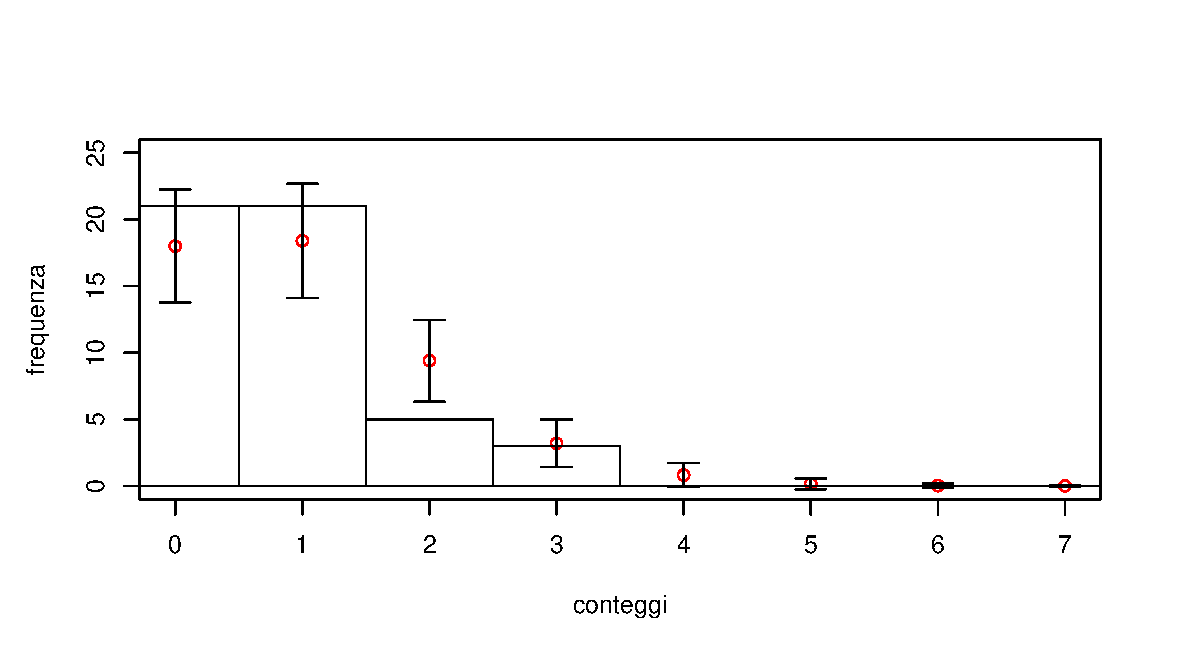
\includegraphics[scale=0.7]{st_uno_nuovo.eps}
\end{figure}

\begin{figure}[H]
\caption{Numero di conteggi per l'intervallo di tempo $\Delta t_2 = \SI{2}{s}$}
\label{fig:istogramma_deltat2}
\centering
\includegraphics[scale=0.7]{ist_due_nuovo.eps}
\end{figure}

\begin{figure}[H]
\caption{Numero di conteggi per l'intervallo di tempo $\Delta t_3 = \SI{3}{s}$}
\label{fig:istogramma_deltat3}
\centering
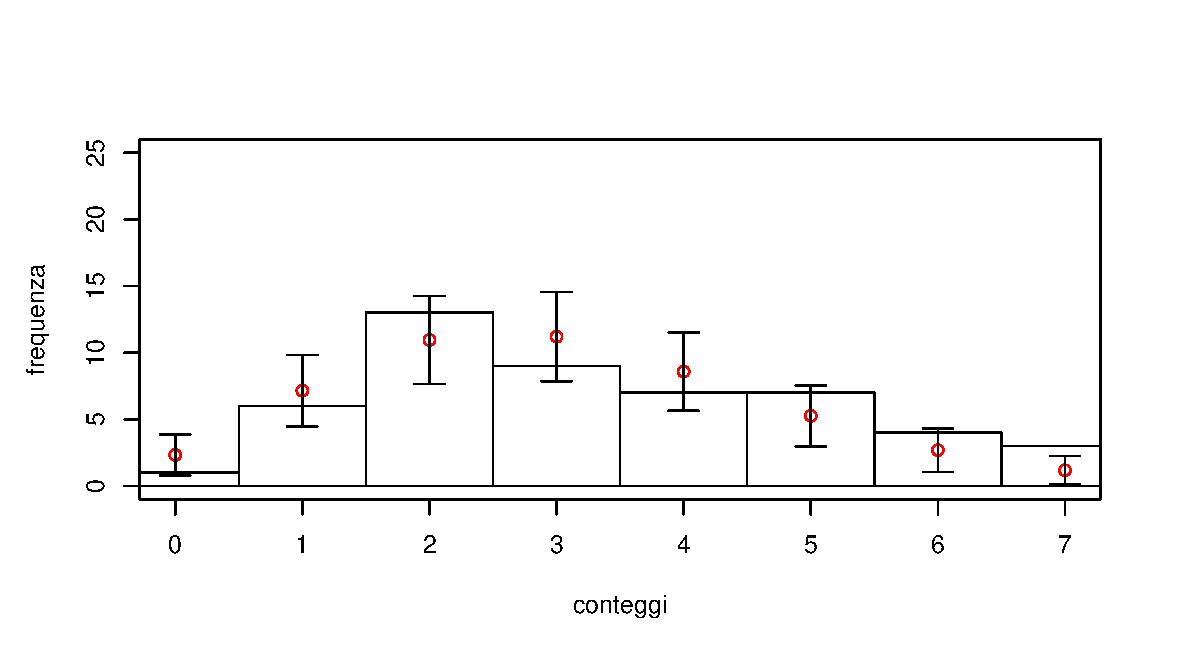
\includegraphics[scale=0.7]{ist_tre_nuovo.eps}
\end{figure}

\begin{figure}[H]
\caption{Numero di conteggi per l'intervallo di tempo $\Delta t_4 = \SI{4}{s}$}
\label{fig:istogramma_deltat4}
\centering
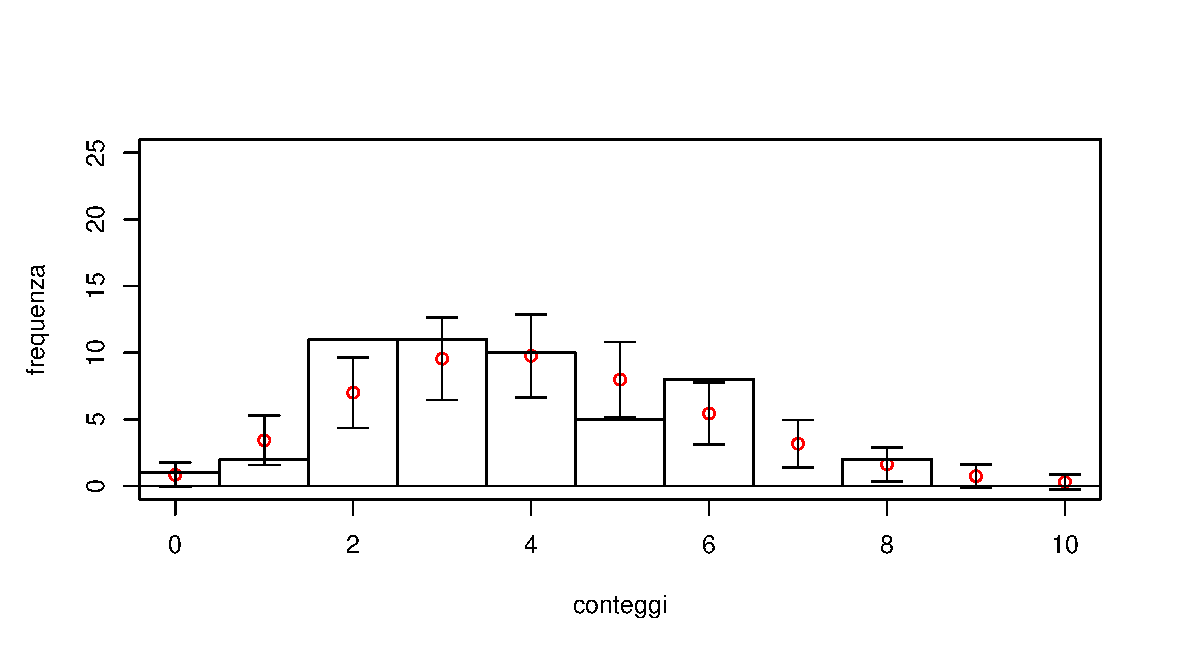
\includegraphics[scale=0.7]{Ist_quattro_nuovo.eps}
\end{figure}

\begin{figure}[H]
\caption{Numero di conteggi per l'intervallo di tempo $\Delta t_5 = \SI{10}{s}$}
\label{fig:istogramma_deltat5}
\centering
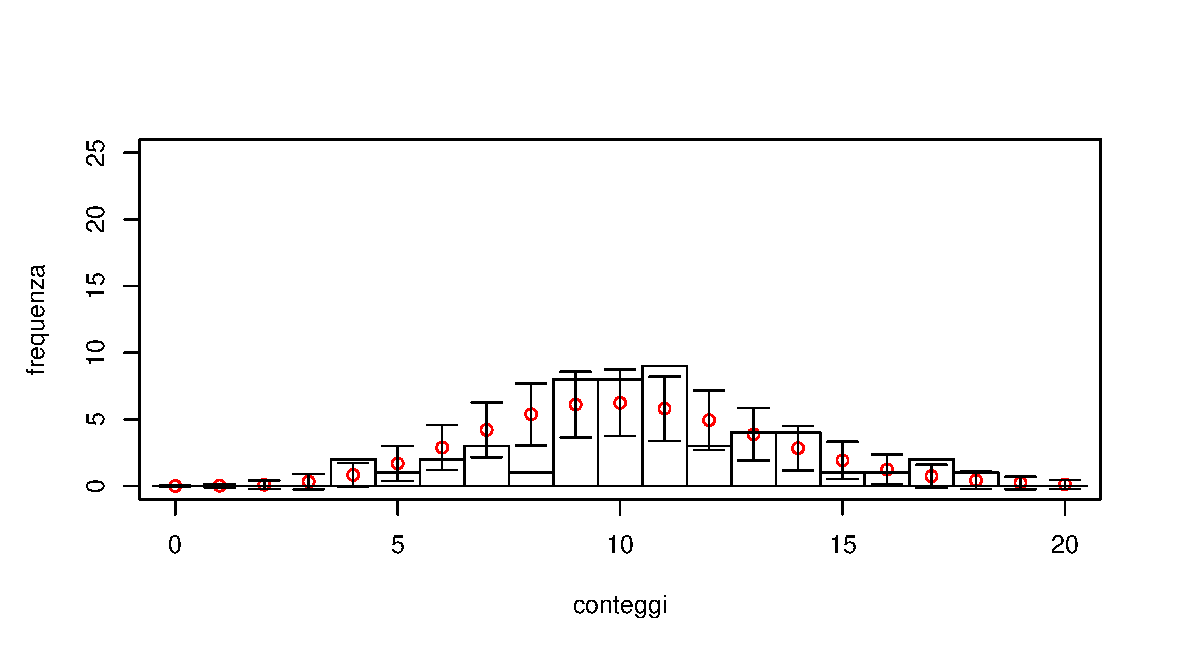
\includegraphics[scale=0.7]{ist_cinque_nuovo.eps}
\end{figure}


\begin{figure}
\caption{Funzione di verosimiglianza per $\Delta T = \SI{1}{s}$}
\label{fig:verosimiglianza1sec}
\centering
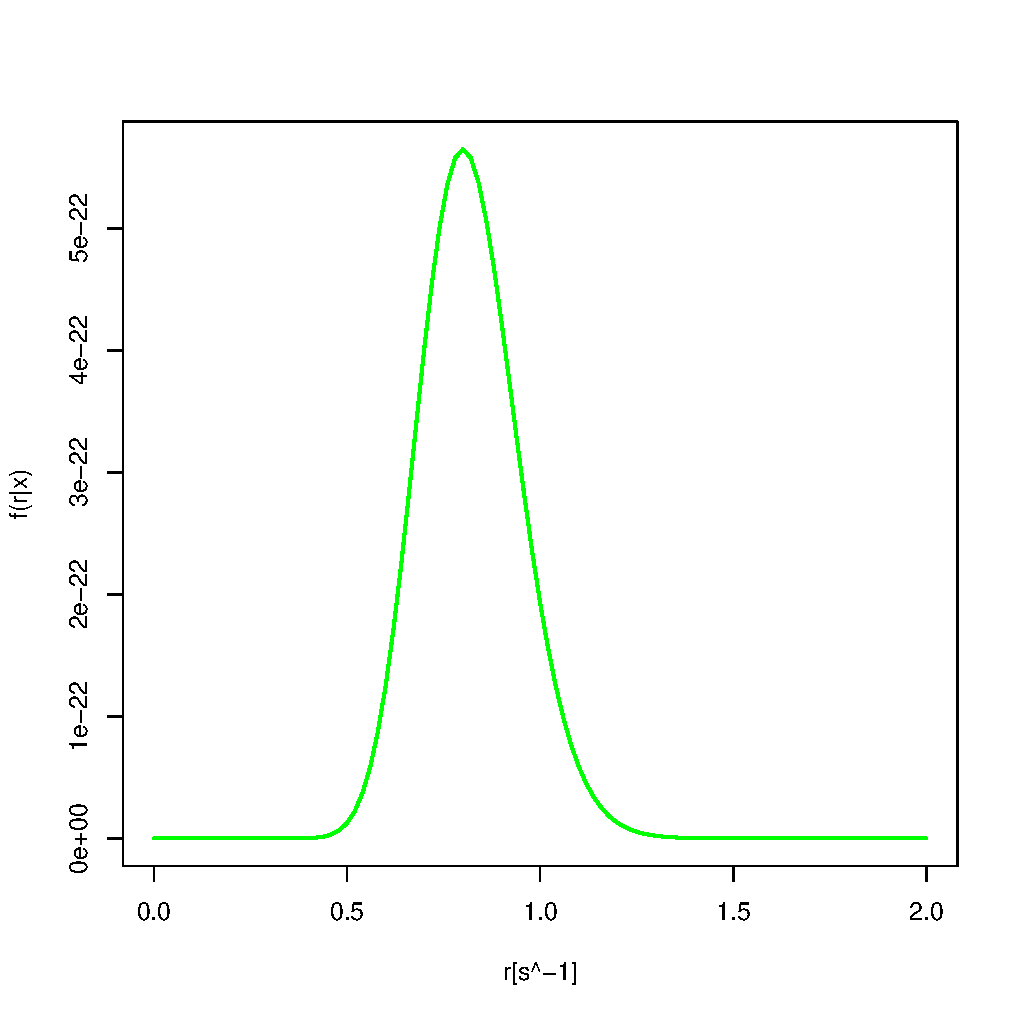
\includegraphics[scale=0.5]{verosimiglianza1sec_nuovo.pdf}
\end{figure}

\begin{figure}
\caption{Funzione di verosimiglianza per $\Delta T = \SI{4}{s}$}
\label{fig:verosimiglianza4sec}
\includegraphics[scale=0.5]{verosimiglainza4sec_nuovo.pdf}
\centering
\end{figure}

\begin{figure}
\caption{Funzione di verosimiglianza per $\Delta T = \SI{599}{s}$}
\label{fig:verosimiglianza600sec}
\centering
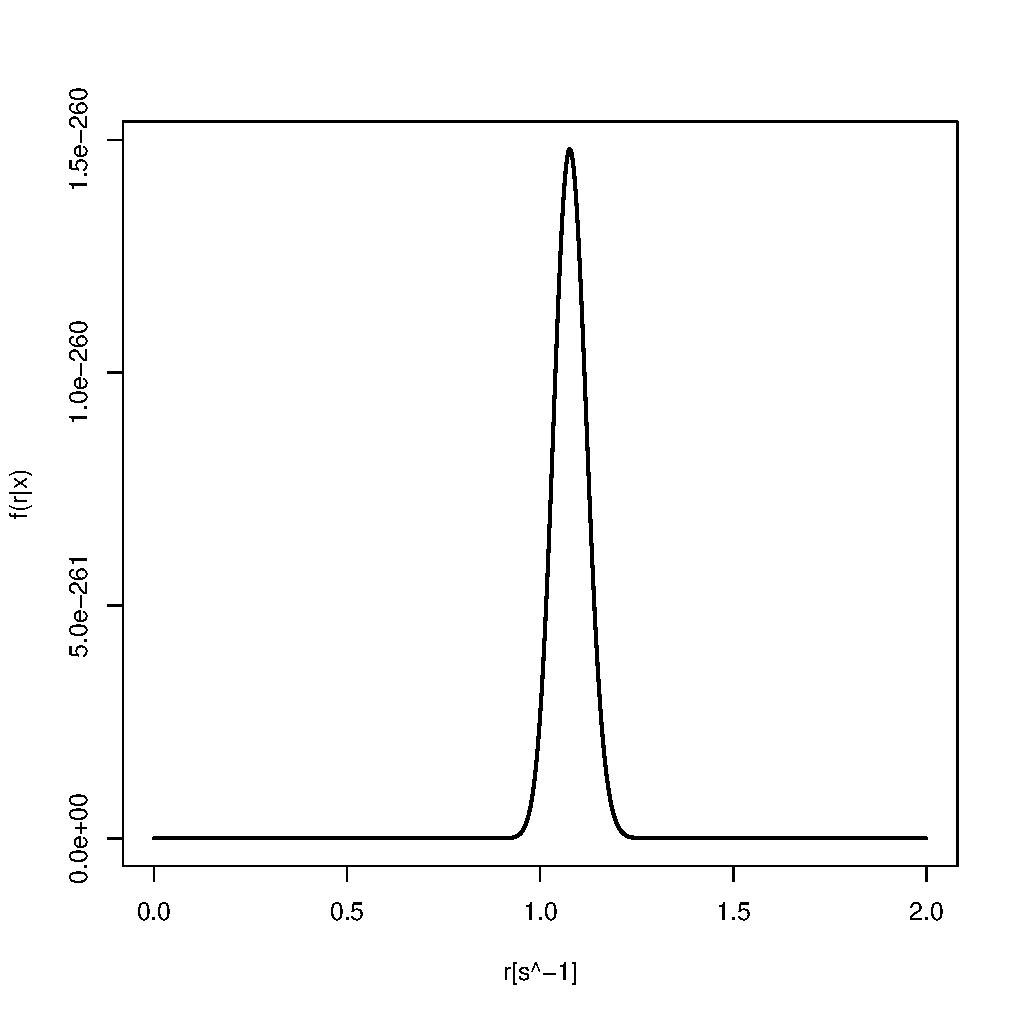
\includegraphics[scale=0.5]{verosimiglianza600sec_nuovo.pdf}
\end{figure}

\begin{figure}
\caption{Funzione di verosimiglianza della combinazione delle misure}
\label{fig:verosimiglianzacombinata}
\centering
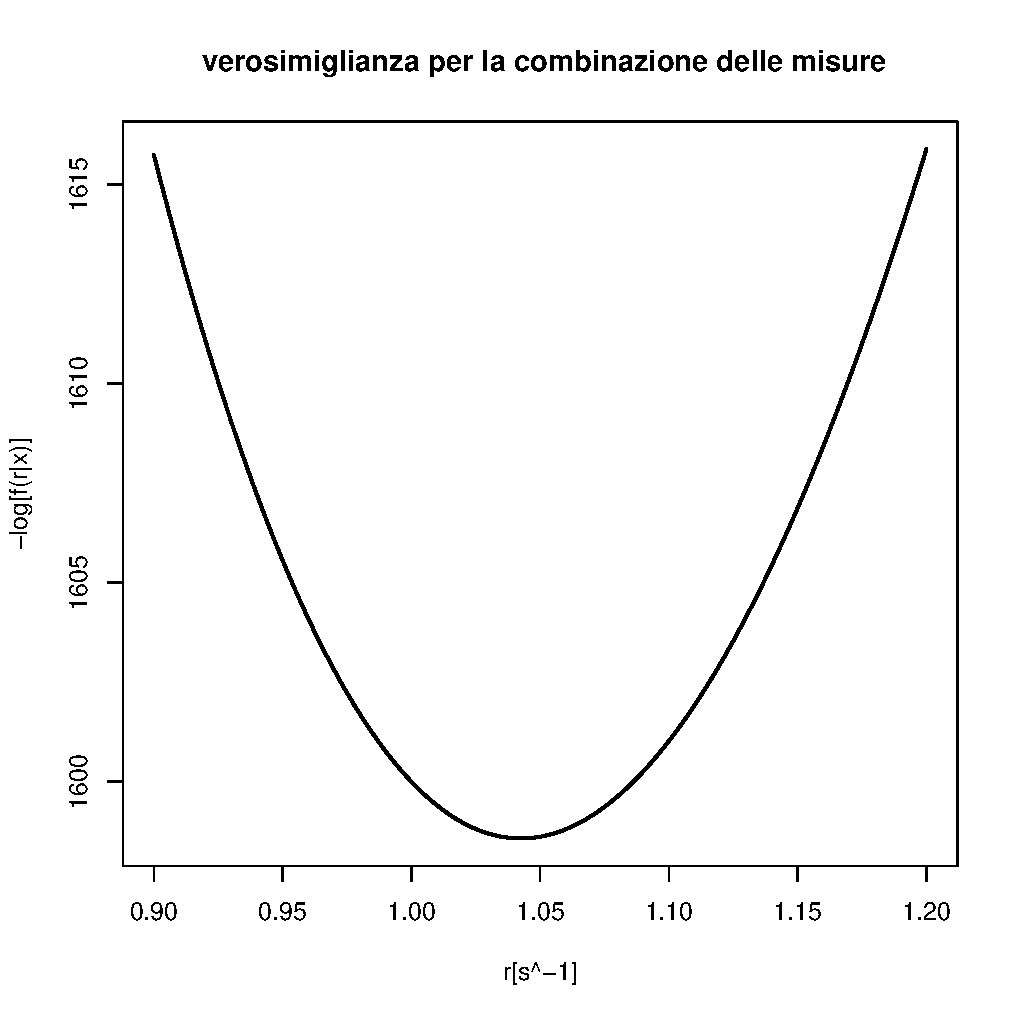
\includegraphics[scale=0.5]{verosimiglianza_comb.pdf}
\end{figure}

%===============CONTEGGI INTEGRALI

\begin{figure}[H]
\caption{Frazione di $0$ conteggi misurati dal contatore Geiger-M\"uller}
\label{fig:0conteggi}
\centering
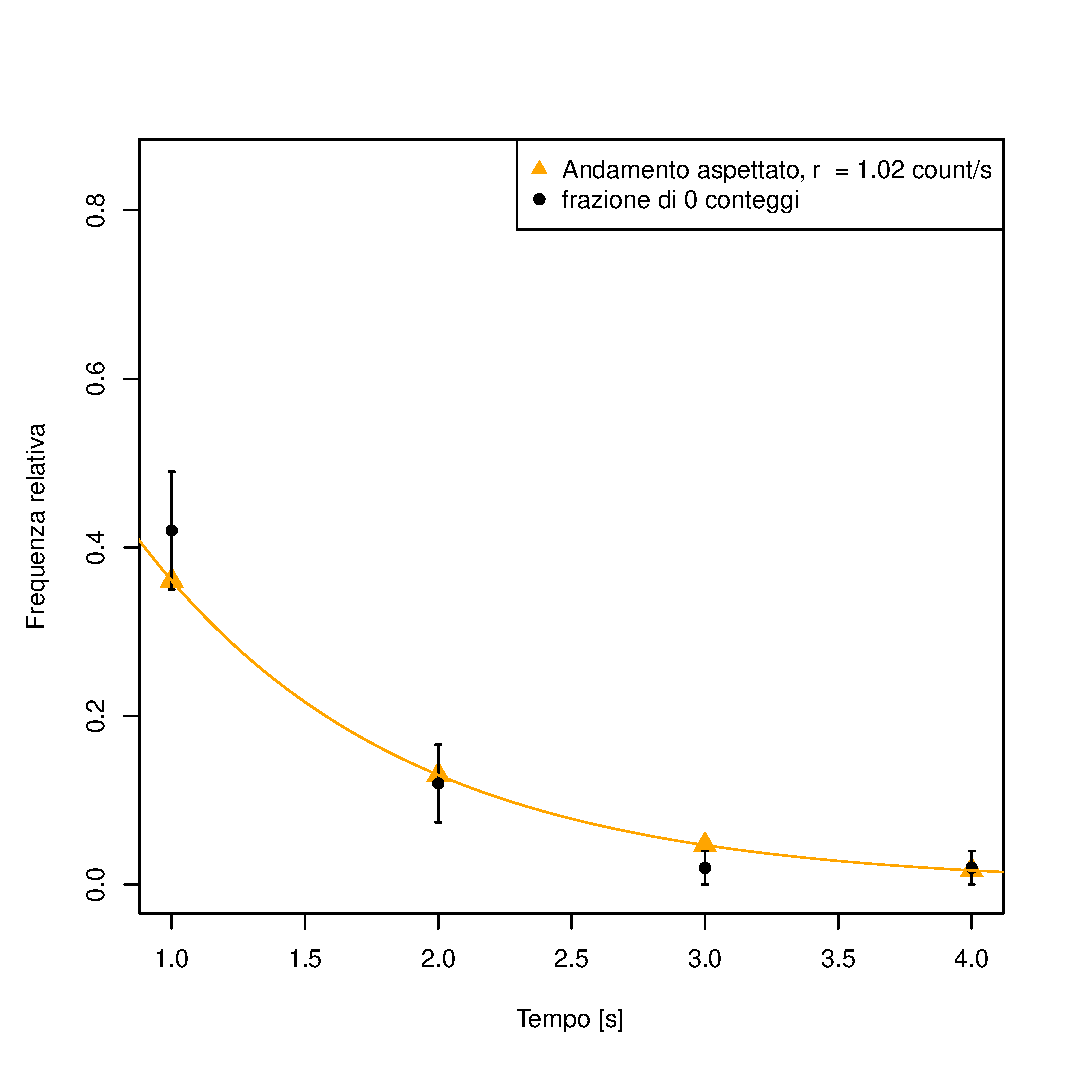
\includegraphics[scale=0.7]{0.eps}
\end{figure}

\begin{figure}[H]
\caption{Frazione di $0$ e di $1$ conteggio misurati dal contatore Geiger-M\"uller}
\label{fig:0+1conteggi}
\centering
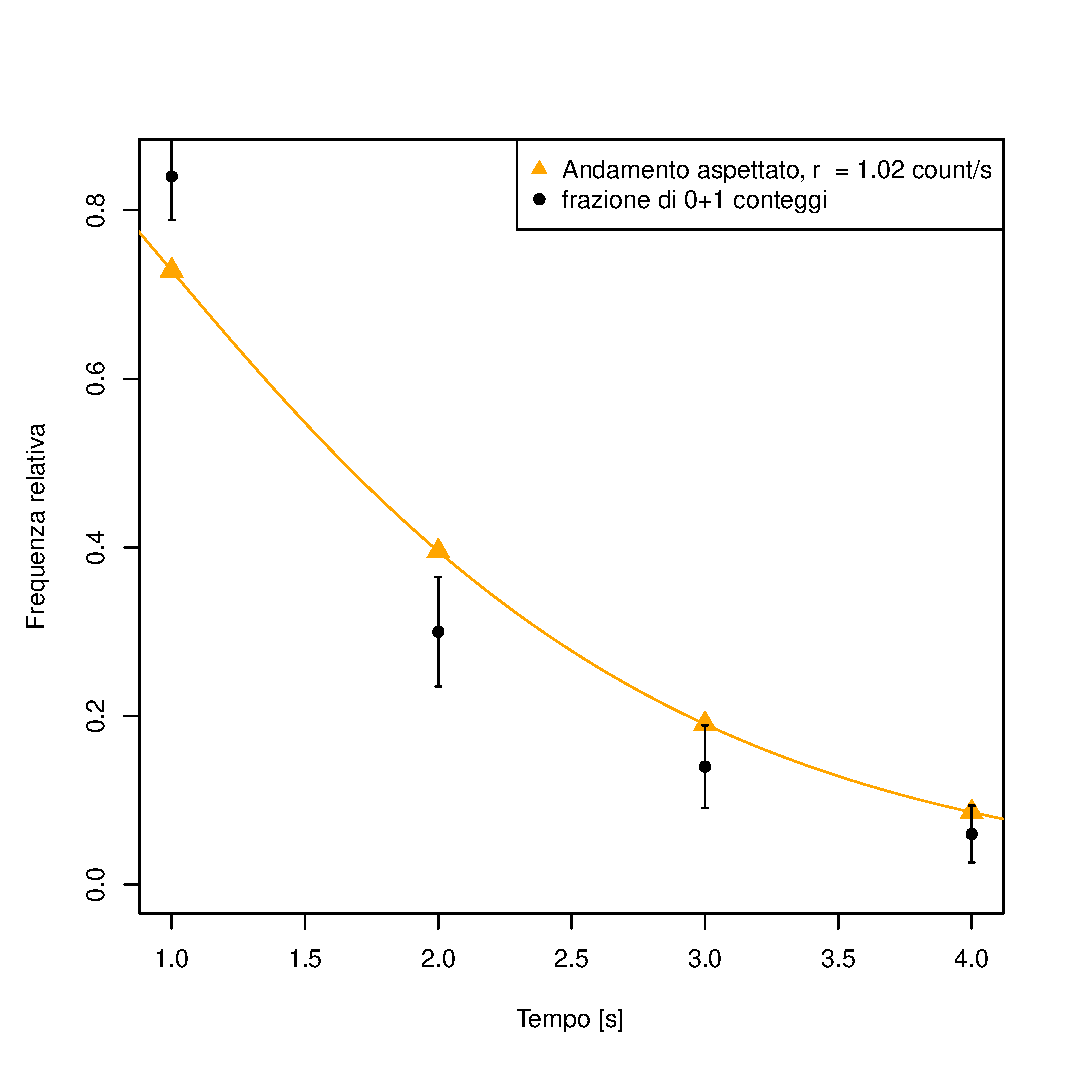
\includegraphics[scale=0.7]{0+1.eps}
\end{figure}

\pagebreak
%============PALLINOMETRO
\subsection{Pallinometro}

\begin{table}[H]
\caption{Conteggi registrati per i bin con il pallinometro orizzontale}
\label{tab:palli_orizzontale}
\centering
\begin{tabular}{ccccc}
  \hline
 & Bin & 33 chiodi & 25 chiodi & 17 chiodi \\ 
  \hline
&0 & 0 & 0 & 0 \\  
&1 & 0 & 0 & 0 \\ 
  &2 & 0 & 0 & 0 \\ 
  &3 & 0 & 0 & 0 \\ 
  &4 & 0 & 0 & 0 \\ 
  &5 & 1 & 0 & 0 \\ 
  &6 & 2 & 1 & 0 \\ 
  &7 & 4 & 2 & 0 \\ 
  &8 & 3 & 4 & 1 \\ 
  &9 & 12 & 9 & 1 \\ 
  &10 & 10 & 9 & 3 \\ 
  &11 & 16 & 16 & 6 \\ 
  &12 & 10 & 14 & 9 \\ 
  &13 & 17 & 21 & 15 \\ 
  &14 & 20 & 20 & 19 \\ 
  &15 & 16 & 13 & 24 \\ 
  &16 & 17 & 20 & 23 \\ 
  &17 & 17 & 11 & 34 \\ 
  &18 & 10 & 16 & 21 \\ 
  &19 & 10 & 15 & 18 \\ 
  &20 & 14 & 13 & 17 \\ 
  &21 & 6 & 7 & 4 \\ 
  &22 & 6 & 7 & 3 \\ 
  &23 & 3 & 2 & 2 \\ 
  &24 & 4 & 0 & 0 \\ 
  &25 & 1 & 0 & 0 \\ 
  &26 & 0 & 0 & 0 \\ 
  &27 & 0 & 0 & 0 \\ 
  &28 & 1 & 0 & 0 \\ 
  &29 & 0 & 0 & 0 \\ 
  &30 & 0 & 0 & 0 \\ 
  &31 & 0 & 0 & 0 \\ 
  &32 & 0 & 0 & 0 \\ 
  &33 & 0 & 0 & 0 \\ 
   \hline
\end{tabular}
\end{table}

\begin{figure}[H]
\caption{Conteggi registrati per i bin con pallinometro orizzontale e $33$ file di chiodi}
\label{fig:palli_orizzontale_33}
\centering
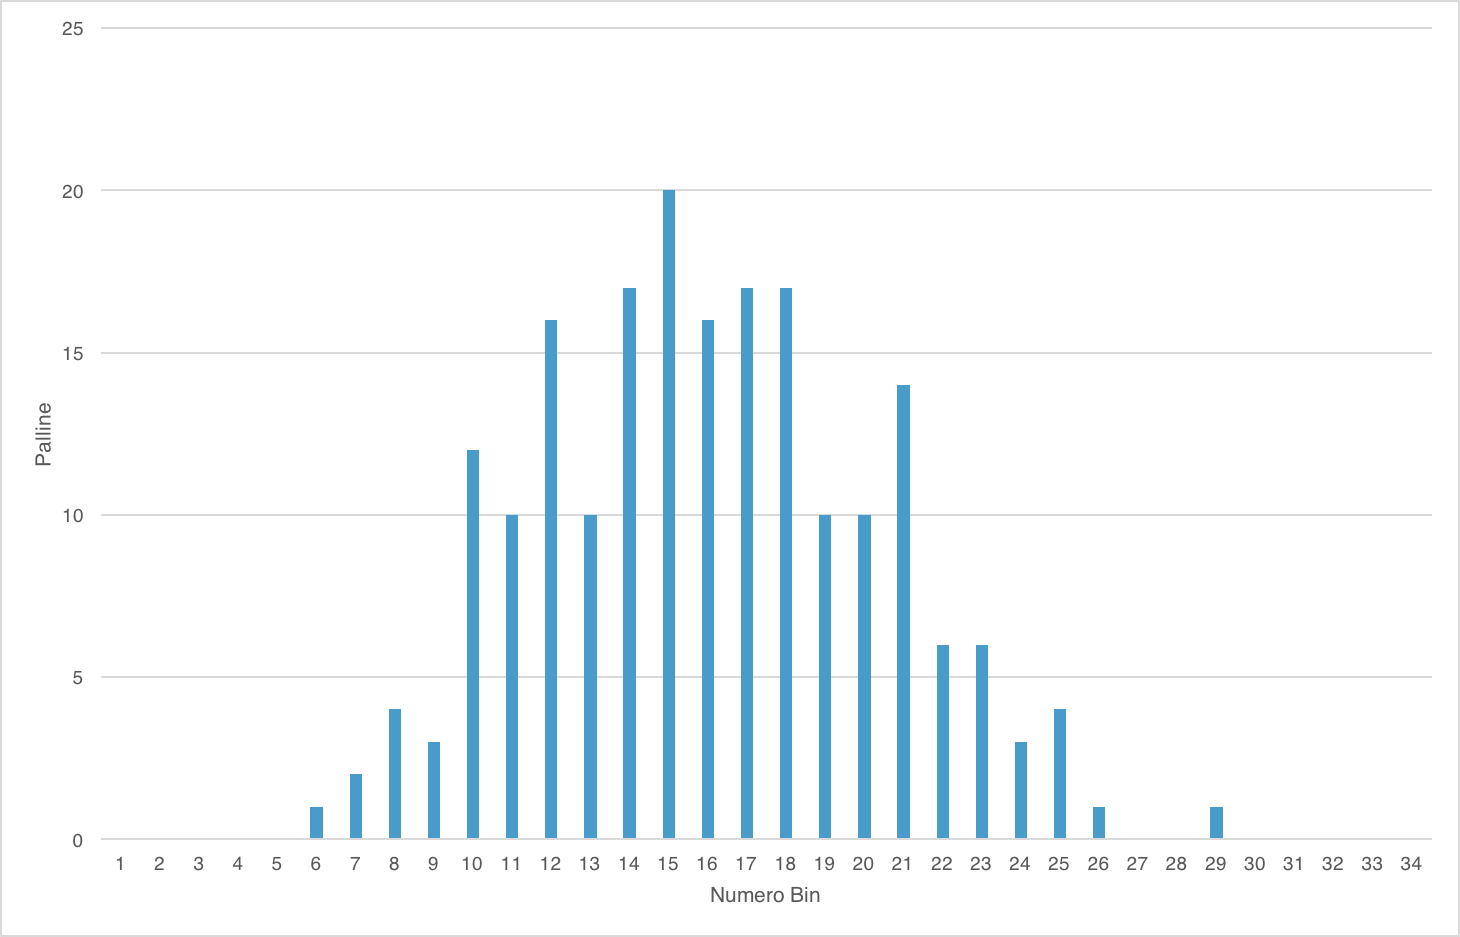
\includegraphics[scale=0.5]{pallinometro_dritto_foro1.png}
\end{figure}
\begin{figure}[H]
\caption{Conteggi registrati per i bin con pallinometro orizzontale e $25$ file di chiodi}
\label{fig:palli_orizzontale_25}
\centering
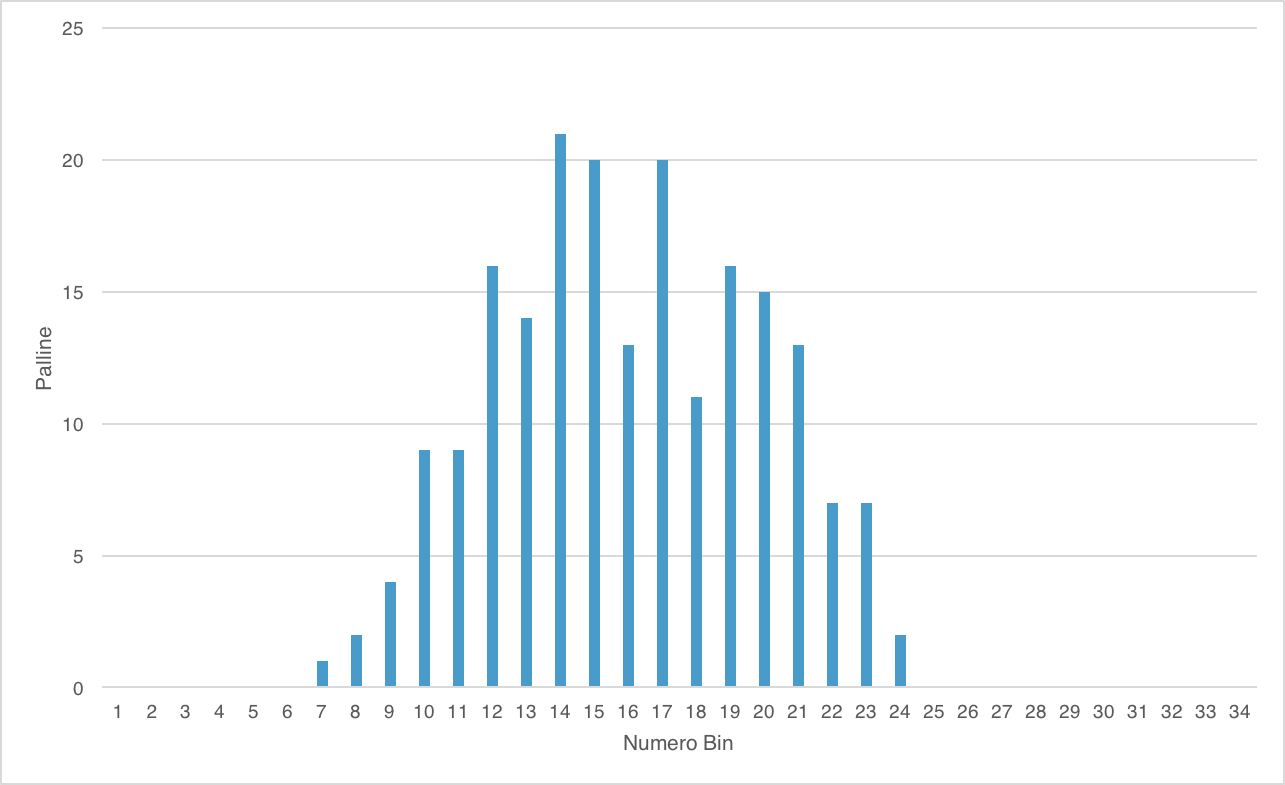
\includegraphics[scale=0.55]{pallinometro_dritto_foro2.png}
\end{figure}
\begin{figure}[H]
\caption{Conteggi registrati per i bin con pallinometro orizzontale e $17$ file di chiodi}
\label{fig:palli_orizzontale_17}
\centering
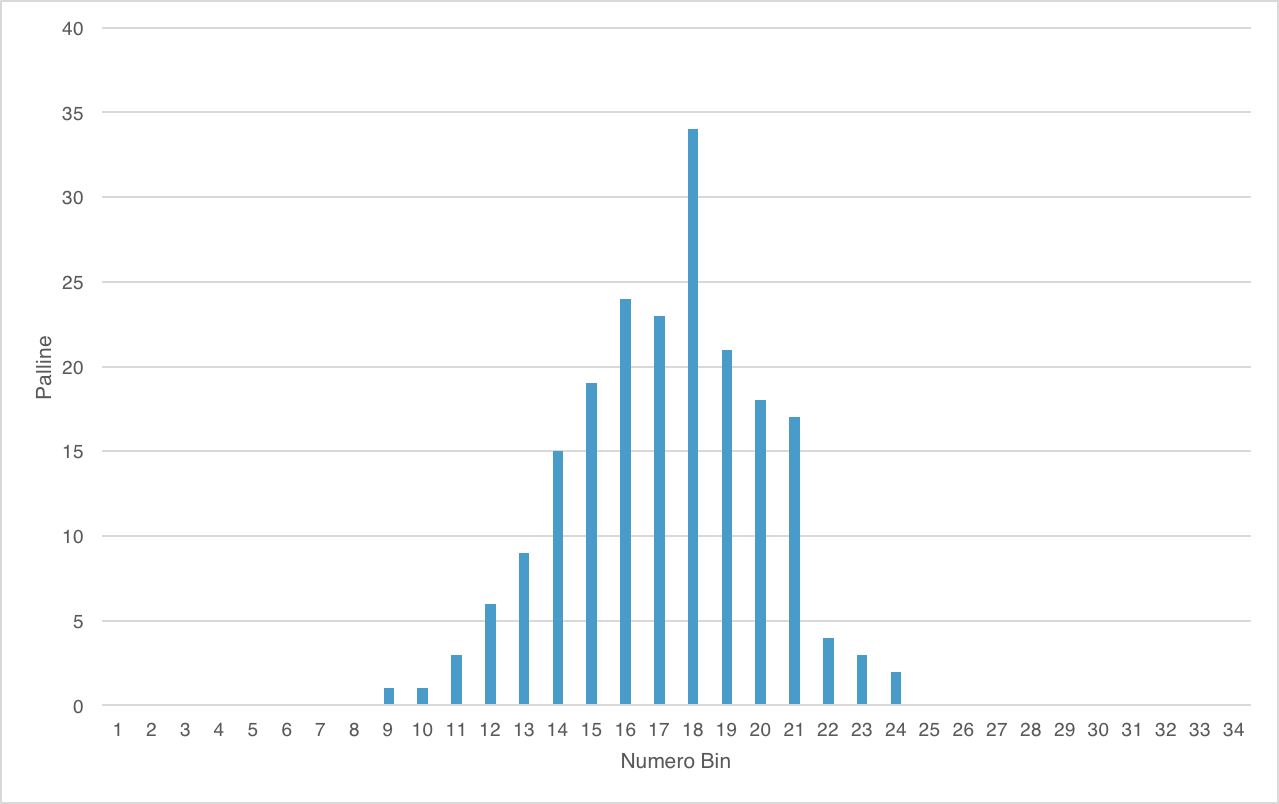
\includegraphics[scale=0.59]{pallinometro_dritto_foro3.png}
\end{figure}



\begin{table}[H]
\caption{Conteggi registrati per i bin con il pallinometro inclinato}
\label{tab:palli_inclinato}
\centering
\begin{tabular}{ccccc}
  \hline
 & Bin & 33 chiodi & 25 chiodi & 17 chiodi \\   
 \hline
&0 & 0 & 0 & 0 \\  
&1 & 0 & 0 & 0 \\ 
&2 & 0 & 0 & 0 \\ 
&3 & 0 & 0 & 0 \\ 
&4 & 0 & 0 & 0 \\ 
&5 & 0 & 0 & 0 \\ 
&6 & 2 & 0 & 0 \\ 
&7 & 0 & 1 & 0 \\ 
&8 & 1 & 1 & 0 \\ 
&9 & 1 & 2 & 0 \\ 
&10 & 4 & 2 & 1 \\ 
  &11 & 2 & 3 & 5 \\ 
  &12 & 9 & 4 & 5 \\ 
  &13 & 7 & 6 & 7 \\ 
  &14 & 14 & 13 & 13 \\ 
  &15 & 13 & 14 & 11 \\ 
  &16 & 15 & 23 & 23 \\ 
  &17 & 16 & 20 & 19 \\ 
  &18 & 11 & 21 & 30 \\ 
  &19 & 16 & 26 & 32 \\ 
  &20 & 16 & 21 & 21 \\ 
  &21 & 14 & 12 & 14 \\ 
  &22 & 12 & 16 & 8 \\ 
  &23 & 10 & 6 & 8 \\ 
  &24 & 18 & 2 & 2 \\ 
  &25 & 7 & 2 & 0 \\ 
  &26 & 4 & 4 & 1 \\ 
  &27 & 4 & 0 & 0 \\ 
  &28 & 1 & 0 & 0 \\ 
  &29 & 0 & 0 & 0 \\ 
  &30 & 1 & 0 & 0 \\ 
  &31 & 2 & 1 & 0 \\ 
  &32 & 0 & 0 & 0 \\ 
  &33 & 0 & 0 & 0 \\ 
   \hline
\end{tabular}
\end{table}

\begin{figure}[H]
\caption{Conteggi registrati per i bin con pallinometro inclinato e $33$ file di chiodi}
\label{fig:palli_inclinato_33}
\centering
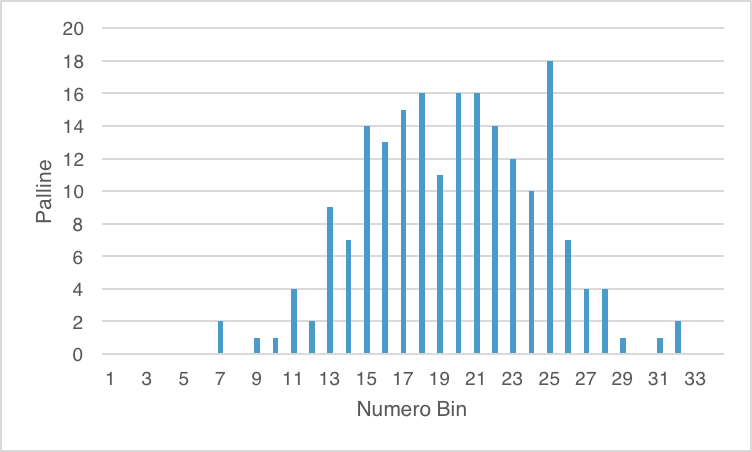
\includegraphics[scale=0.9]{pallinometro_inclinato_foro1.png}
\end{figure}
\begin{figure}[H]
\caption{Conteggi registrati per i bin con pallinometro inclinato e $25$ file di chiodi}
\label{fig:palli_inclinato_25}
\centering
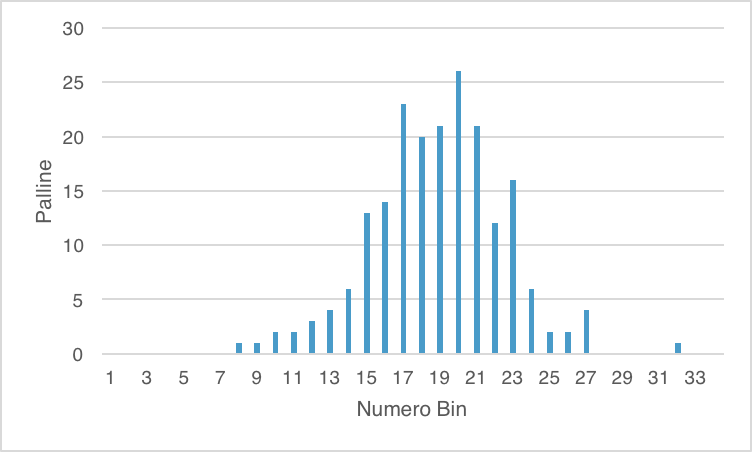
\includegraphics[scale=0.9]{pallinometro_inclinato_foro2.png}
\end{figure}
\begin{figure}[H]
\caption{Conteggi registrati per i bin con pallinometro inclinato e $17$ file di chiodi}
\label{fig:palli_inclinato_17}
\centering
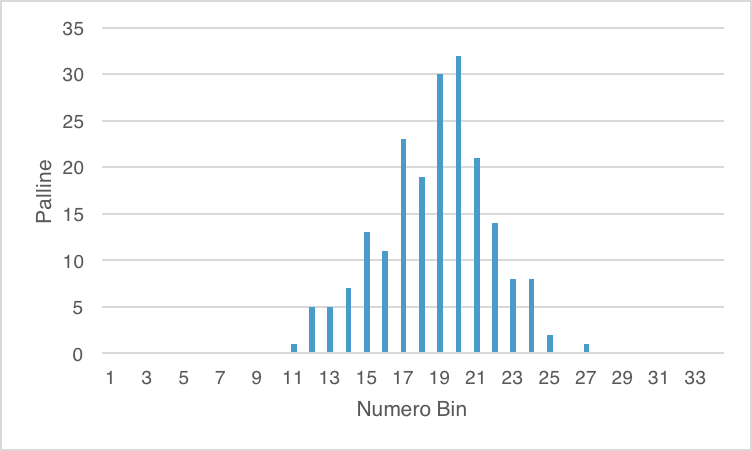
\includegraphics[scale=0.9]{pallinometro_inclinato_foro3.png}
\end{figure}


\begin{table}[H]
\caption{Frequenze relative dei singoli bin con il pallinometro orizzontale}
\label{tab:freq_rel_orizzontale}
\centering
\begin{tabular}{ccccc}
\hline
 & Bin & 33 chiodi & 25 chiodi & 17 chiodi \\   
  \hline
&0 & 0.00 & 0.00 & 0.00 \\
&1 & 0.00 & 0.00 & 0.00 \\ 
 & 2 & 0.00 & 0.00 & 0.00 \\ 
  &3 & 0.00 & 0.00 & 0.00 \\ 
  &4 & 0.00 & 0.00 & 0.00 \\ 
  &5 & 0.01 & 0.00 & 0.00 \\ 
  &6 & 0.01 & 0.01 & 0.00 \\ 
  &7 & 0.02 & 0.01 & 0.00 \\ 
  &8 & 0.01 & 0.02 & 0.01 \\ 
  &9 & 0.06 & 0.04 & 0.01 \\ 
  &10 & 0.05 & 0.04 & 0.01 \\ 
  &11 & 0.08 & 0.08 & 0.03 \\ 
  &12 & 0.05 & 0.07 & 0.04 \\ 
  &13 & 0.09 & 0.10 & 0.07 \\ 
  &14 & 0.10 & 0.10 & 0.10 \\ 
  &15 & 0.08 & 0.07 & 0.12 \\ 
  &16 & 0.09 & 0.10 & 0.12 \\ 
  &17 & 0.09 & 0.06 & 0.17 \\ 
  &18 & 0.05 & 0.08 & 0.10 \\ 
  &19 & 0.05 & 0.07 & 0.09 \\ 
  &20 & 0.07 & 0.07 & 0.09 \\ 
  &21 & 0.03 & 0.04 & 0.02 \\ 
  &22 & 0.03 & 0.04 & 0.01 \\ 
  &23 & 0.01 & 0.01 & 0.01 \\ 
  &24 & 0.02 & 0.00 & 0.00 \\ 
  &25 & 0.01 & 0.00 & 0.00 \\ 
  &26 & 0.00 & 0.00 & 0.00 \\ 
  &27 & 0.00 & 0.00 & 0.00 \\ 
  &28 & 0.01 & 0.00 & 0.00 \\ 
  &29 & 0.00 & 0.00 & 0.00 \\ 
  &30 & 0.00 & 0.00 & 0.00 \\ 
  &31 & 0.00 & 0.00 & 0.00 \\ 
  &32 & 0.00 & 0.00 & 0.00 \\ 
  &33 & 0.00 & 0.00 & 0.00 \\ 
   \hline
\end{tabular}
\end{table}



\begin{table}[H]
\caption{Frequenze relative dei singoli bin con il pallinometro inclinato}
\label{tab:freq_rel_inclinato}
\centering
\begin{tabular}{ccccc}
  \hline
 & Bin & 33 chiodi & 25 chiodi & 17 chiodi \\   
 \hline
&0 & 0.00 & 0.00 & 0.00 \\ 
&1 & 0.00 & 0.00 & 0.00 \\ 
  &2 & 0.00 & 0.00 & 0.00 \\ 
  &3 & 0.00 & 0.00 & 0.00 \\ 
  &4 & 0.00 & 0.00 & 0.00 \\ 
  &5 & 0.00 & 0.00 & 0.00 \\ 
  &6 & 0.01 & 0.00 & 0.00 \\ 
  &7 & 0.00 & 0.01 & 0.00 \\ 
  &8 & 0.01 & 0.01 & 0.00 \\ 
  &9 & 0.01 & 0.01 & 0.00 \\ 
  &10 & 0.02 & 0.01 & 0.01 \\ 
  &11 & 0.01 & 0.01 & 0.03 \\ 
  &12 & 0.04 & 0.02 & 0.03 \\ 
  &13 & 0.04 & 0.03 & 0.04 \\ 
  &14 & 0.07 & 0.07 & 0.07 \\ 
  &15 & 0.07 & 0.07 & 0.06 \\ 
  &16 & 0.07 & 0.12 & 0.12 \\ 
  &17 & 0.08 & 0.10 & 0.10 \\ 
  &18 & 0.06 & 0.10 & 0.15 \\ 
  &19 & 0.08 & 0.13 & 0.16 \\ 
  &20 & 0.08 & 0.10 & 0.10 \\ 
  &21 & 0.07 & 0.06 & 0.07 \\ 
  &22 & 0.06 & 0.08 & 0.04 \\ 
  &23 & 0.05 & 0.03 & 0.04 \\ 
  &24 & 0.09 & 0.01 & 0.01 \\ 
  &25 & 0.04 & 0.01 & 0.00 \\ 
  &26 & 0.02 & 0.02 & 0.01 \\ 
  &27 & 0.02 & 0.00 & 0.00 \\ 
  &28 & 0.01 & 0.00 & 0.00 \\ 
  &29 & 0.00 & 0.00 & 0.00 \\ 
  &30 & 0.01 & 0.00 & 0.00 \\ 
  &31 & 0.01 & 0.01 & 0.00 \\ 
  &32 & 0.00 & 0.00 & 0.00 \\ 
  &33 & 0.00 & 0.00 & 0.00 \\ 
   \hline
\end{tabular}
\end{table}

\begin{figure}[H]
\caption{Simulazione con \emph{Palli2000} del pallinometro orizzontale con $33$ file di chiodi}
\label{fig:palli2000_orizzontale_33}
\centering
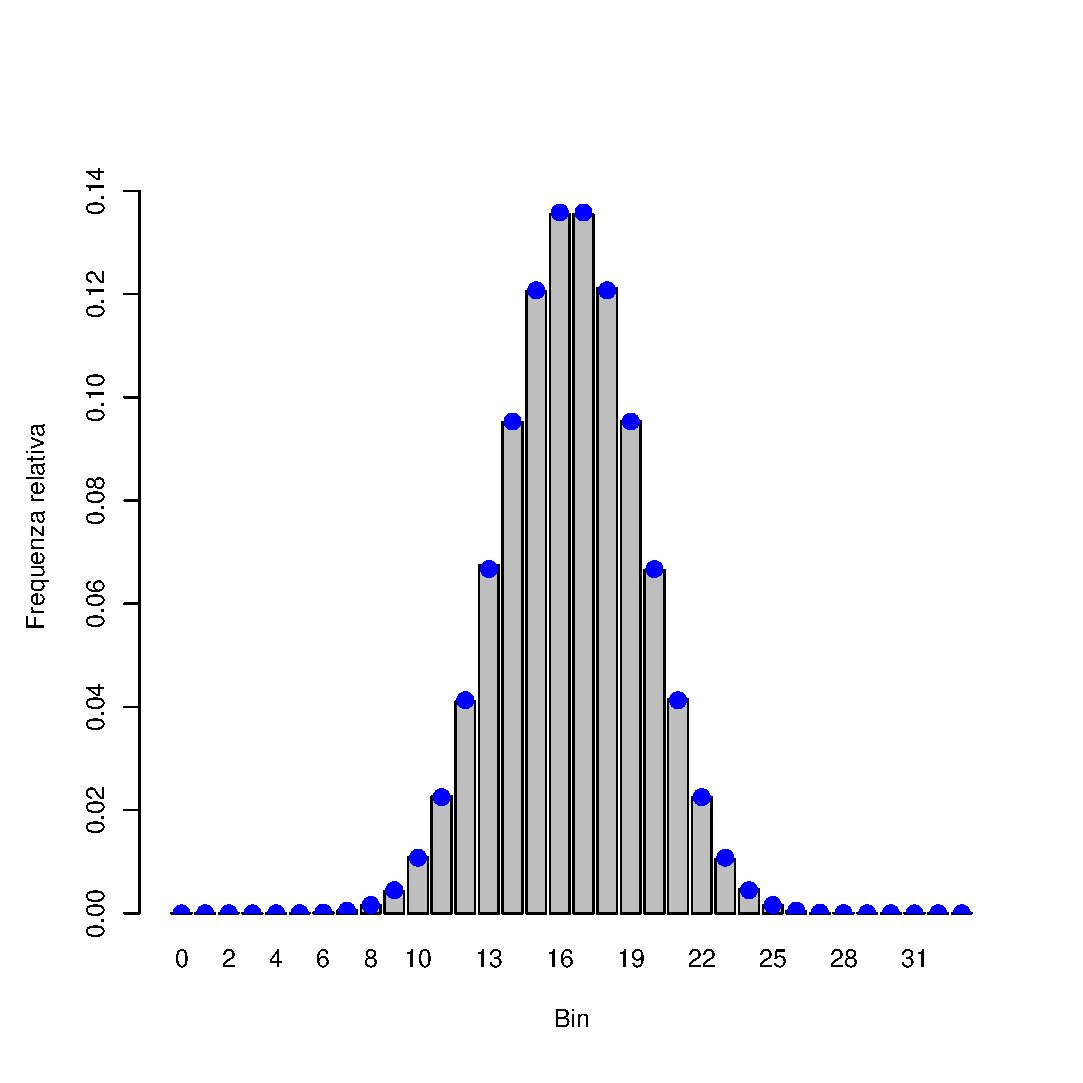
\includegraphics[scale=0.5]{palli2000_orizz_1.eps}
\end{figure}
\begin{figure}[H]
\caption{Simulazione con \emph{Palli2000} del pallinometro orizzontale con $25$ file di chiodi}
\label{fig:palli2000_orizzontale_25}
\centering
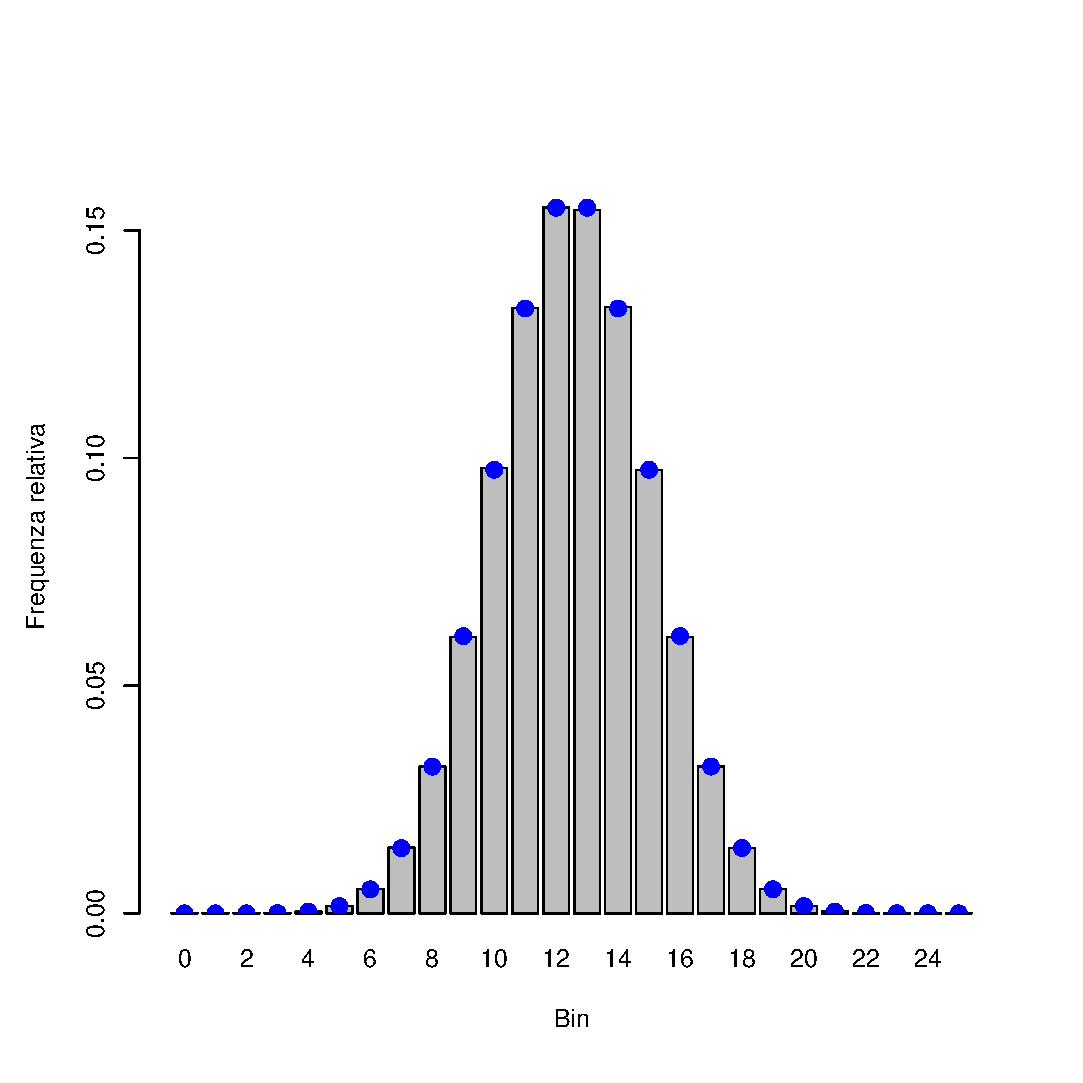
\includegraphics[scale=0.5]{palli2000_orizz_2.eps}
\end{figure}
\begin{figure}[H]
\caption{Simulazione con \emph{Palli2000} del pallinometro orizzontale con $17$ file di chiodi}
\label{fig:palli2000_orizzontale_17}
\centering
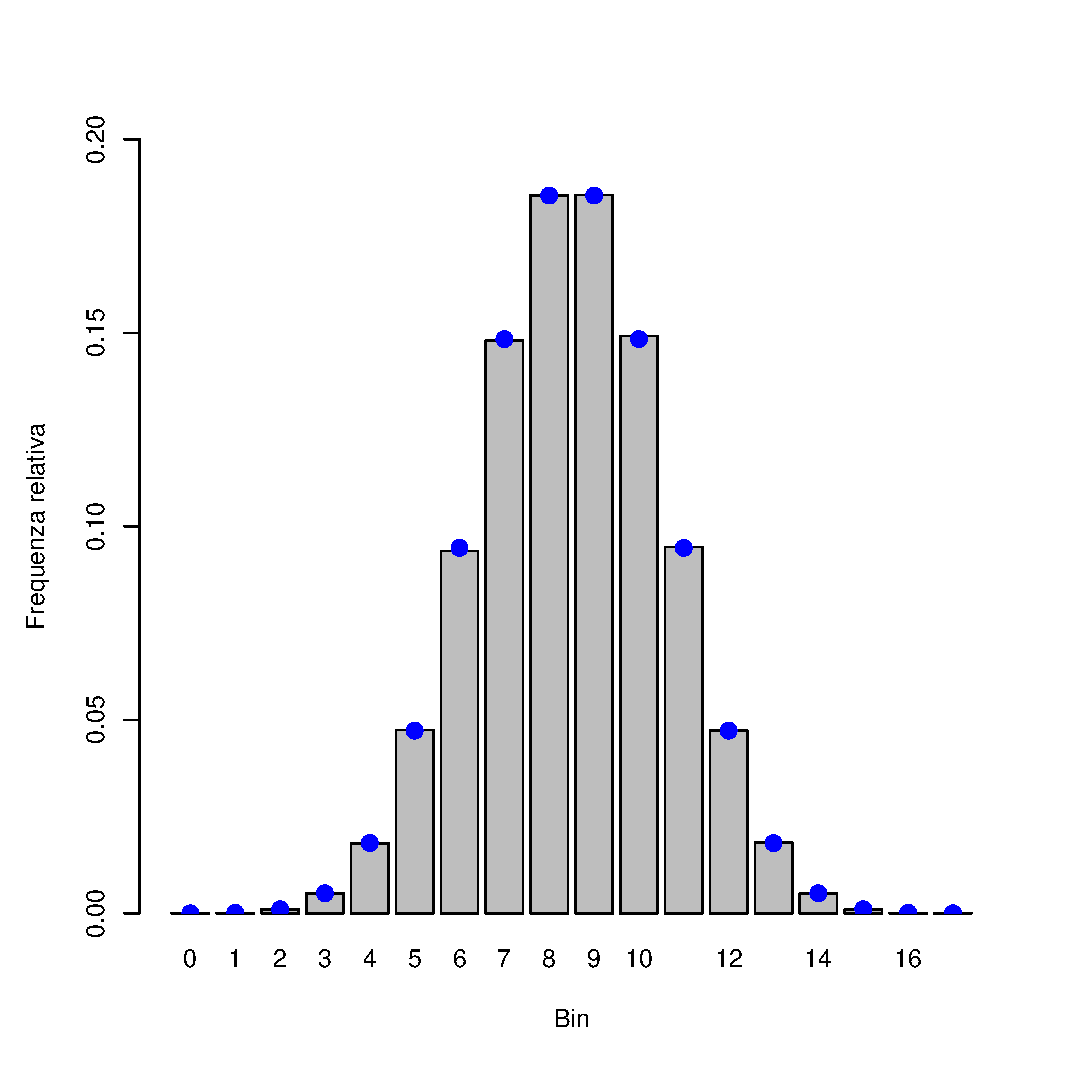
\includegraphics[scale=0.5]{palli2000_orizz_3.eps}
\end{figure}



\begin{figure}[H]
\caption{Simulazione con \emph{Palli2000} del pallinometro inclinato con $33$ file di chiodi}
\label{fig:palli2000_inclinato_33}
\centering
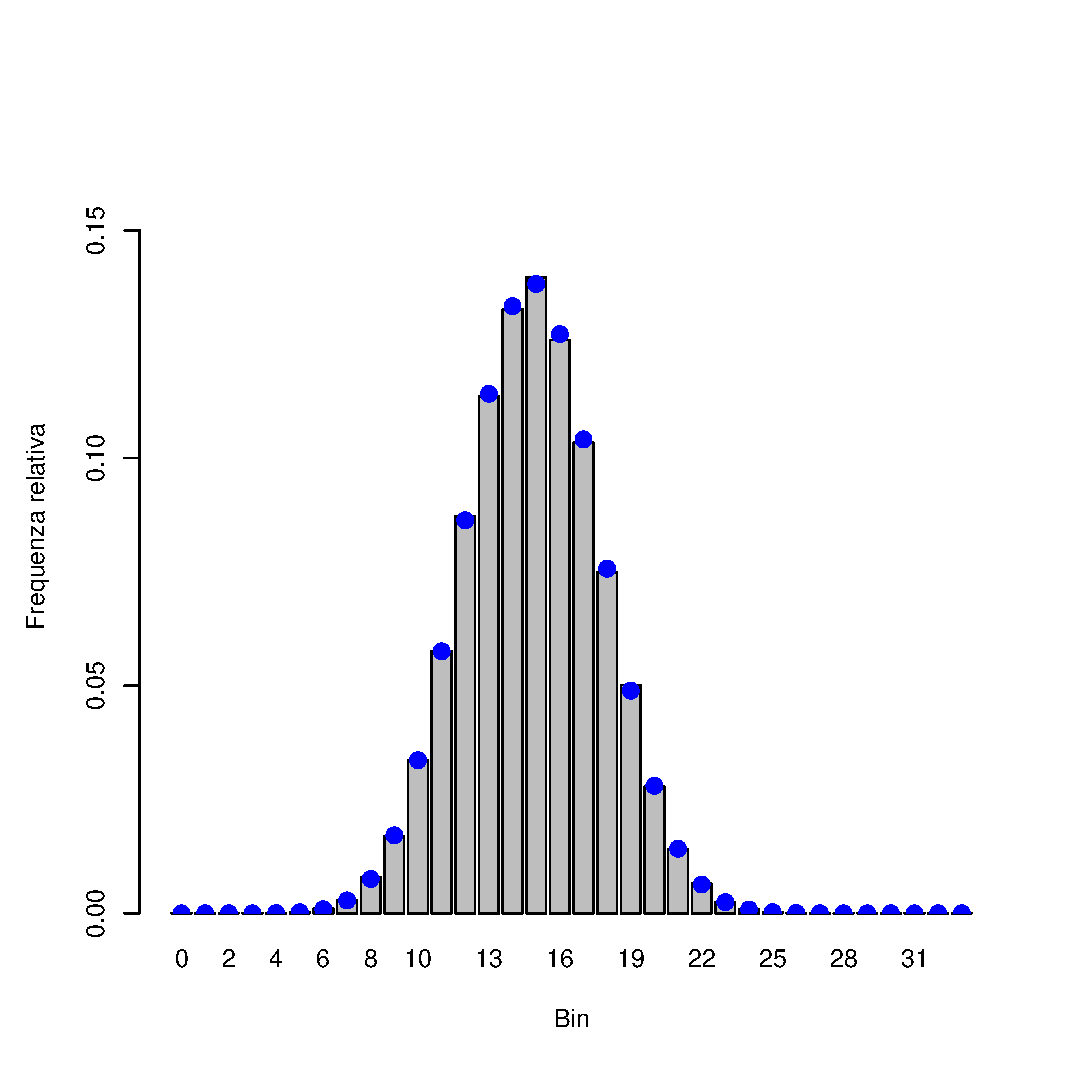
\includegraphics[scale=0.5]{palli200_inclinato_1.eps}
\end{figure}
\begin{figure}[H]
\caption{Simulazione con \emph{Palli2000} del pallinometro inclinato con $25$ file di chiodi}
\label{fig:palli2000_inclinato_25}
\centering
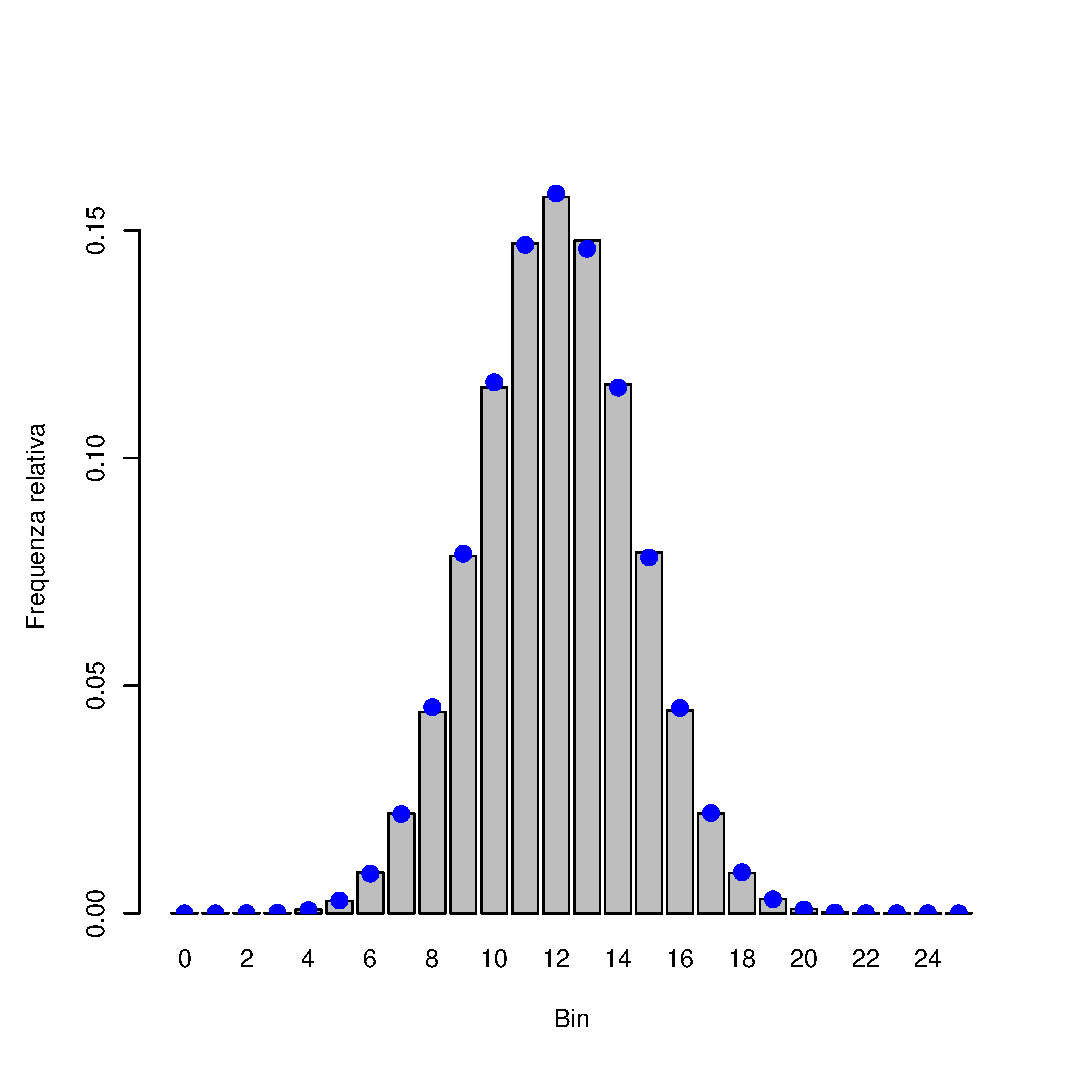
\includegraphics[scale=0.5]{palli200_inclinato_2.eps}
\end{figure}
\begin{figure}[H]
\caption{Simulazione con \emph{Palli2000} del pallinometro inclinato con $17$ file di chiodi}
\label{fig:palli2000_inclinato_17}
\centering
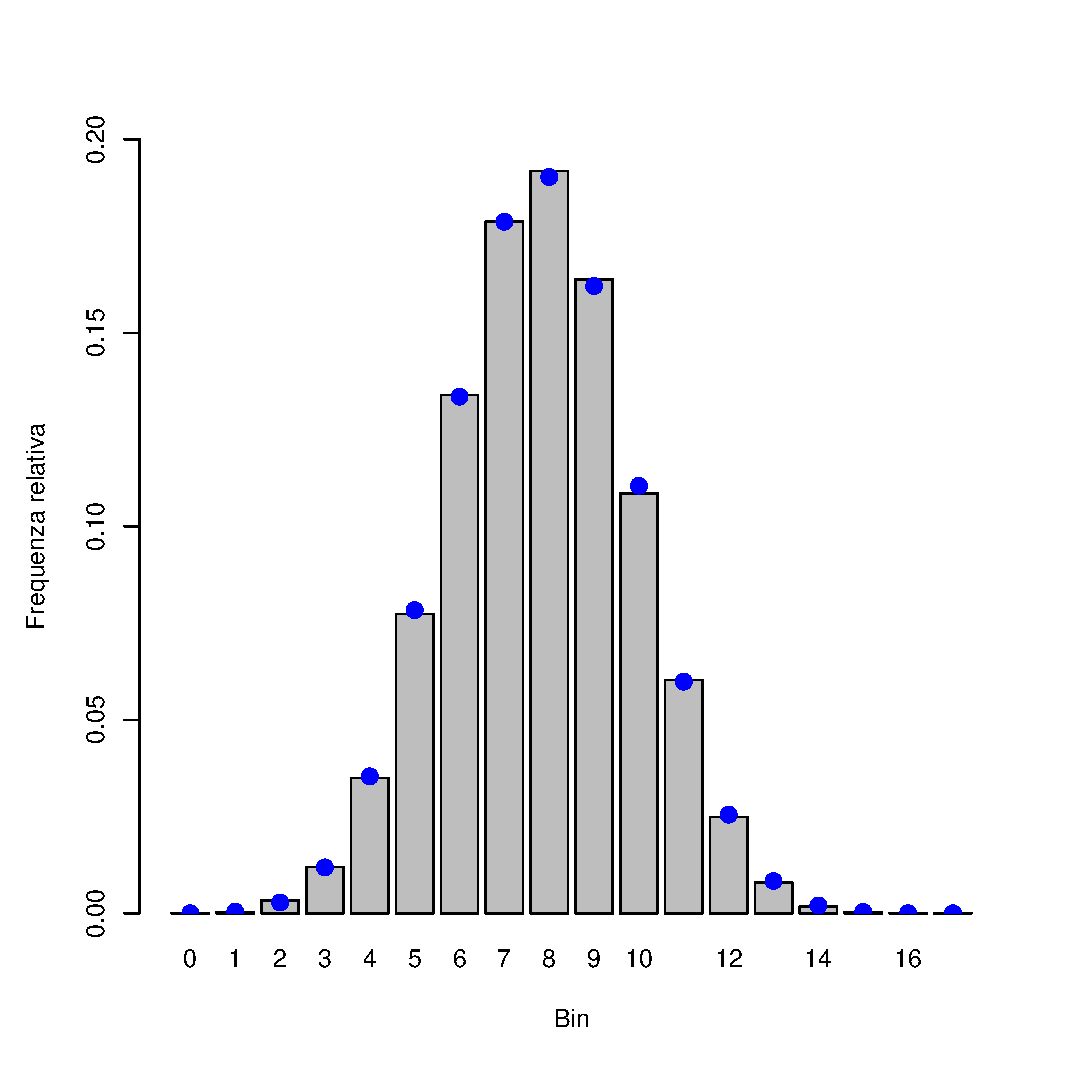
\includegraphics[scale=0.5]{palli200_inclinato_3.eps}
\end{figure}

\begin{figure}[H]
\caption{Simulazione con C di un pallinometro con distribuzione gaussiana della probabilità  di cadere a destra per ogni chiodo}
\label{}
\centering
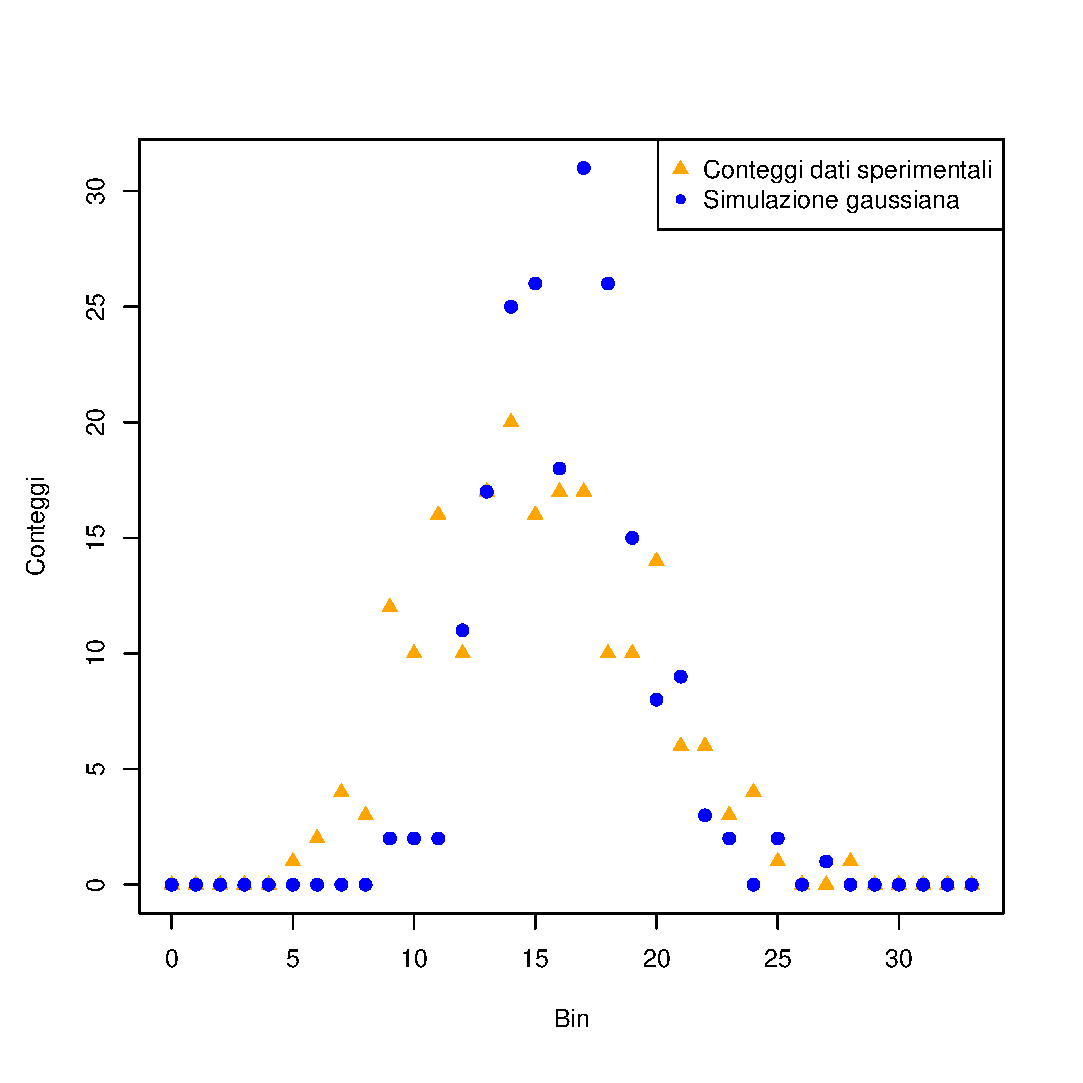
\includegraphics[scale=0.5]{lollo.eps}
\end{figure}

\begin{codice_c}[caption={Simulazione di un pallinometro con distribuzione gaussiana della probabilità  di cadere a destra per ogni chiodo}, label={list:codice}][H]
#include <stdio.h>
#include <stdlib.h>
#include <math.h>
#include <time.h>
#define nMin 10 //palline
#define nMax 1000000
#define xMin 0.
#define xMax 1.
#define M 34 //cellette (compresa la numero 0)
#define p 0.5 //probabilità 
#define MU 0.5
#define SIGMA 0.15
double casual(double min, double max);
double fdist(double x, double mu, double sigma);
double hitAndMiss(double mu, double sigma);
int main() {
  int n = 0;
  int chk = 0;
  int i = 0;
  int k = 0;
  int d = 0;
  int celletta[M] = {0};
  FILE *pf;
  srand48(time(0));
  printf("Questo programma simula il funzionamento di un
pallinometro con %d file di chiodi e dunque %d cellette.\nInserisci
il numero di palline, compreso tra %d e %d: ", M-1, M, nMin, nMax);
  do {
  chk = scanf("%d", &n);
  if (chk != 1) {
    char buffer[255];
    scanf("%s", buffer);
    printf("Inserisci nuovamente il numero: ");
  }
  } while((chk != 1) || (n<nMin) || (n>nMax));
  for(i=0;i<n;i++) {
    for(k=0;k<M-1;k++) {
      if(casual(0.,1.)>hitAndMiss(MU,SIGMA)) {
        d++;
} }
    celletta[d]++;
d = 0; }
  pf = fopen("palli2000.dat", "w");
for(k=0;k<M;k++) {
    printf("Celletta\t%d:\t%d\n", k, celletta[k]);
    fprintf(pf, "%d\t%d\n", k, celletta[k]);
}
  fclose(pf);
}
double casual(double min, double max) {
  double diff = max - min;
  return min + diff * lrand48() / RAND_MAX;
}
double fdist(double x, double mu, double sigma) {
  return (1/(sigma*sqrt(2*M_PI))) * exp(-(pow((x-mu),2)) /
(2*pow(sigma,2)));
}
double hitAndMiss(double mu, double sigma) {
  double x = 0.;
  double y = 0.;
  double f = 0.;
  double xDef = 0.;
  double F = fdist(mu,mu,sigma);
  do {
    x = casual(xMin, xMax);
    y = casual(0., F);
    f = fdist(x, mu, sigma);
    if(y < f) {
      xDef = x;
    }
  } while(y >= f);
  return xDef;
}
\end{codice_c}









\end{document}
